\documentclass[12pt]{article}

\usepackage{ishn}

\makeindex[intoc]

\begin{document}

\hypersetup{pageanchor=false}
\begin{titlepage}
	\begin{center}
		\vspace*{1em}
		\Huge
		\textbf{III Functional Analysis}

		\vspace{1em}
		\large
		Ishan Nath, Michaelmas 2024

		\vspace{1.5em}

		\Large

		Based on Lectures by Dr. Andr\'as Zs\'ak

		\vspace{1em}

		\large
		\today
	\end{center}
	
\end{titlepage}
\hypersetup{pageanchor=true}

\tableofcontents

\newpage

% lecture 1

\setcounter{section}{-1}

\section{Introduction}%
\label{sec:intro}

Allen has good notes.

Books include Bollob\'as, Rudin, S.J. Taylor (measure theory), Rudin again and Murphy.

\subsection{Overview}%
\label{sub:over}

The course is structured as follows.
\begin{enumerate}[label=Chapter \arabic*.]
	\item Hahn-Banach extension theorems.
	\item Dual spaces of $L_p(\mu)$ and $C(K)$.
	\item Weak topologies.
	\item Convexity and Krein-Milman theorem.
	\item Banach algebras.
	\item Holomorphic functional calculus.
	\item $C^\ast$-algebras.
	\item Borel functional calculus and spectral theory.
\end{enumerate}

\newpage

\section{Hahn-Banach Extension Theorems}%
\label{sec:hb_ext}

Let $X$ be a normed space. The \emph{dual space}\index{dual space} $X^\ast$ of $X$ is
\[
	X^\ast = \{f : X \to \text{scalars} \mid f \text{ linear, continuous (or bounded)}\}.
\]
This is a normed space in the operator norm. For $f \in X^\ast$,
\[
	\|f\| = \sup \{|f(x)| \mid x \in B_X\},
\]
where $B_X$ is the unit ball in $X$, i.e. $\{x \in X \mid \|x\| \leq 1\}$. We also have $S_X = \{x \in X \mid \|x\| = 1\}$, the unit sphere.

Recall that $X^\ast$ is a Banach space.

\begin{exbox}
	$\ell_p^\ast \cong \ell_q$, for $1 \leq p < \infty$, $1 < q \leq \infty$, and $1/p + 1/q = 1$.

	We also have $c_0^\ast \cong \ell_1$.

	Also if $H$ is a Hilbert space, then $H^\ast \cong H$, by the Riesz representation theorem. This is conjugate linear in the complex case.
\end{exbox}

\begin{definition}
	We write $X \sim Y$ if NVS's $X$ and $Y$ are isomorphic, so there exists a linear bijection $T : X \to Y$ where $T$ and $T^{-1}$ are bounded.

If $X, Y$ are both Banach spaces, and $T : X \to Y$ is a continuous linear bijection, then $T^{-1}$ is continuous by the open mapping theorem.

	Write $X \cong Y$ if $X$ and $Y$ are isometrically isomorphic, i.e. there exists a surjective linear map $T : X \to Y$ such that $T$ is isometric, i.e. $\|Tx\| = \|x\|$.

	Note this automatically implies $T$ is a linear bijection, and $T^{-1}$ is isometric.

	For a normed space $X$, and $x \in X$, $f \in X^\ast$ we write
	\[
	\langle x, f \rangle = f(x).
	\]
	This is bilinear, and $|\langle x, f\rangle| = |f(x)| \leq \|f\| \cdot \|x\|$. When $X$ is a Hilbert space, $X^\ast$ is identified with $X$, and $\langle \cdot, \cdot \rangle$ is the inner product.
\end{definition}

\begin{definition}
	Let $X$ be a real vector space. A functional $p : X \to \mathbb{R}$ is:
	\begin{enumerate}[(i)]
		\item \emph{positive homogeneous}\index{positive homogeneous} if $p(tx) = tp(x)$ for all $x \in X$, $t \geq 0$.
		\item \emph{subadditive}\index{subadditive} if $p(x + y) \leq p(x) + p(y)$.
	\end{enumerate}
\end{definition}

\begin{theorem}[Hahn-Banach]
	Let $X$ be a real vector space, and $p : X \to \mathbb{R}	$ be a positive homogeneous, subadditive functional on $X$. Let $Y$ be a subspace of $X$, and $g : Y \to \mathbb{R}$ be linear such that $g(y) \leq p(y)$ for all $y \in Y$.

	Then there exists linear $f : X \to \mathbb{R}$ such that $f|_Y = g$, and $f(x) \leq p(x)$ for all $x \in X$.
\end{theorem}

To prove this, we need Zorn's lemma, and the theory of posets. Let $(P, \leq)$ be a poset.

For $A \subseteq P$, $x \in P$, say $x$ is an \emph{upper bound} for $A$ if $a \leq x$ for all $a \in A$. For $C \subseteq P$, say $C$ is a \emph{chain} if $\leq$ is a linear order on $C$. Say $x \in P$ is a \emph{maximal element} if, for all $y \in P$, $x \leq y$ implies $y = x$.

\begin{theorem}[Zorn's lemma]
	If $P$ is a non-empty poset and every non-empty chain in $P$ has an upper bound, then $P$ has a maximal element.
\end{theorem}

\begin{proofbox}
	Consider the poset given by pairs $(Z, h)$, where $Z$ is a subspace of $X$ containin $Y$, and $h : Z \to \mathbb{R}$ linear, with $h|_Y = g$, and $h(z) \leq p(z)$.

	Here $(Z_1, h_1) \leq (Z_2, h_2)$ if $Z_1 \subseteq Z_2$ and $h_2 |_{Z_1} = h_1$. This can be checked to be a partial order.

	Now we check our conditions. First $P \neq \emptyset$ as $(Y, g) \in P$. Moreover, given a non-empty chain $C = \{(Z_i, h_I) \mid i \in I\}$ in $P$, we can set $Z = \bigcup_{i \in I} Z_i$, and define $h : Z \to \mathbb{R}$ by $h|_{Z_i} = h_i$. Then $(Z, h) \in P$ and is an upper bound for $C$.

	Thus by Zorn's, $P$ has a maximal element $(W, f)$. Now we need to show that $W = X$, and we will be done.

	Assume not. Fix $z \in X \setminus W$, and a real number $\alpha \in \mathbb{R}$. Define $f_1 : W_1 = W + \mathbb{R}\cdot z \to \mathbb{R}$ by
	\[
	f_1(w + \lambda z) = f(w) + \lambda \alpha.
	\]
	Then $f_1$ is linear, and $f_1|_W = f$. To be done, we need to choose $\alpha$ so that $f_1(w_1) \leq p(w_1)$ for all $w_1 \in W_1$.

	Thus we need
	\begin{align*}
		f(w) + \lambda \alpha &\leq p(w + \lambda z) \\
		\iff f(w) + \alpha &\leq p(w + z) \\
		f(w) - \alpha &\leq p(w - z),
	\end{align*}
	for all $w \in W$. This means
	\[
	f(x) - p(x - z) \leq \alpha \leq p(y + z) - f(y),
	\]
	which is true if and only if
	\[
	f(x) - p(x - z) \leq p(y + z) - f(y),
	\]
	for all $x, y \in W$, by taking $\alpha$ to be the supremum of the left hand side as $x$ ranges over $W$. But this is true as
	\[
	f(x) + f(y) = f(x + y) \leq p(x + y) = p(x - z + y + z) \leq p(x - z) + p(y + z),
	\]
	for all $x, y \in W$.
\end{proofbox}

%lecture 2

\begin{definition}
	A \emph{seminorm}\index{seminorm} on a real or complex vector space $X$ is a functional $p : X \to \mathbb{R}$ such that:
	\begin{enumerate}[(i)]
		\item $p(x) \geq 0$, for all $x \in X$.
		\item $p(\lambda x) = |\lambda|p(x)$, for all scalars $\lambda$, and for all $x \in X$.
		\item $p(x + y) \leq p(x) + p(y)$ for all $x, y \in X$.
	\end{enumerate}
\end{definition}

This is the definition of the norm, without requiring $p(x) = 0 \implies x = 0$.

Of course, any seminorm is positive heterogeneous, and subadditive.

\begin{theorem}[Hahn-Banach]
	Let $X$ be a real or complex vector space, and $p$ a seminorm on $X$. Let $Y$ be a subspace of $X$, and $g$ be a linear functional on $Y$ such that $|g(y)| \leq p(y)$, for all $y \in Y$.

	Then there exists linear functional $f$ on $X$, such that $f|_Y = g$, and $|f(x)| \leq p(x)$ for all $x \in X$.
\end{theorem}

\begin{proofbox}
	We split into two cases, the real and the complex case.

	In the real case, we have $g(y) \leq |g(y)| \leq p(y)$ for all $y \in Y$, so by the first version of Hahn-Banach, there exists a linear map $f : X \to \mathbb{R}$ such that $f|_Y = g$ and $f(x) \leq p(x)$.

	We are almost done, except we need $|f(x)| \leq p(x)$. Here we use the fact that $p$ is a seminorm, so
	\[
	-f(x) = f(-x) \leq p(-x) = p(x).
	\]
	Hence $|f(x)| \leq p(x)$.

	Now we start with the complex case. Splitting into real and imaginary parts does not work, as $f, g$ real linear does not imply $f + ig$ complex linear. To do this, we show the following claim:

	\textbf{Claim:} For any real-linear $h_1 : X \to \mathbb{R}$, there is a unique complex linear $h : X \to \mathbb{C}$ such that $\Re(h) = h_1$.

	We start with uniqueness. If $h_1 = \Re(h)$, then for $x \in X$,
	\begin{align*}
		h(x) &= h_1(x) + i \Im(h(x)) \\
		     &= -i h(ix) = -i (h_1(ix) + i \Im(h(ix))).
	\end{align*}
	So, $\Im(H(x)) = - h_1(ix)$, and thus
	\[
	h(x) = h_1(x) - i h_1(ix).
	\]
	For existence, we just check this $h$ defined above works, and it does (clearly real-linear, just need to check multiplication by $i$ is correct).

	We return back to our proof. Let $g_1 = \Re(g) : Y \to \mathbb{R}$, which is real-linear. For $y \in Y$, note
	\[
	|g_1(y)| \leq |g(y)| \leq p(y).
	\]
	By the real case, there exists a real linear $f_1 : X \to \mathbb{R}$ such that $f_1|_Y = g_1$, and $|f_1(x)| \leq p(x)$ for all $x \in X$.

	By the claim, $f_1 = \Re(f)$ for unique complex-linear functions $f : X \to \mathbb{C}$, and note
	\[
	\Re(f|_Y) = f_1|_Y = g_1 = \Re(g).
	\]
	Therefore by uniqueness, $f|_Y = g$. We are almost done apart form domination. Note that for $x \in X$, $|f(x)| = \lambda f(x)$, for some $\lambda \in \mathbb{C}$, $|\lambda| = 1$. Then,
	\begin{align*}
		|f(x)| &= f(\lambda x) = f_1(\lambda x) + i \Im (f(\lambda x)) \\
		       &= f_1(\lambda x) \leq p(\lambda x) = |\lambda| p(x) = p(x).
	\end{align*}
\end{proofbox}

\begin{remark}
	For a complex vector space $X$, let $X_{\mathbb{R}}$ be the real vector space obtained from $X$ by restricting scalar multiplication to the reals.

	If $X$ is a complex normed space, then $f \mapsto \Re(f)$ on $(X^\ast)_{\mathbb{R}} \to (X_{\mathbb{R}})^\ast$ is an isometric isomorphism.
\end{remark}

\begin{corollary}
	Let $X$ be a real or complex vector space, and let $p$ be a seminorm on $X$. Then for any $x_0 \in X$, there exists a linear functional $f$ on $X$ such that $f(x_0) = p(x_0)$, and $|f(x)| \leq p(x)$, for all $x \in X$.
\end{corollary}

\begin{proofbox}
	Let $Y = \spn\{x_0\}$, and define $g$ on $Y$ be
	\[
	g(\lambda x_0) = \lambda p(x_0).
	\]
	Then $g$ is linear on $Y$, and
	\[
	|g(\lambda x_0)| = |\lambda|p(x_0) = p(\lambda x_0),
	\]
	for all scalars $\lambda$. Thus by Hahn-Banach, there exists a linear functional $f$ on $X$ such that $f|_Y = g$, and $|f(x)| \leq p(x)$. So $f(x_0) = g(x_0) = p(x_0)$.
\end{proofbox}

\begin{theorem}[Hahn-Banach]
	Let $X$ be a real or complex normed space.
	\begin{enumerate}[\normalfont(i)]
		\item Given a subspace $Y$ of $X$ and $g \in Y^\ast$, here exists $f \in X^\ast$ such hat $f|_Y = g$, and $\|f\| = \|g\|$.
		\item For $x_0 \in X \setminus \{0\}$, here exists $f \in S_{X^\ast}$ such that $f(x_0) = \|x_0\|$.
	\end{enumerate}
\end{theorem}

\begin{proofbox}
	

	(i) Apply previous Hahn-Banach with $p(x) = \|g\| \|x\|$. Then for $y \in Y$,
	\[
	|g(y)| \leq \|g\| \cdot \|y\| = p(y).
	\]
	Hence there exists a linear functional $f$ on $X$ such that $f|_Y = g$, and
	\[
	|f(x)| \leq p(x) = \|g\| \cdot \|x\|.
	\]
	Therefore, $f \in X^\ast$, and $\|f\| = \|g\|$. Since $f$ extends $g$, $\|f\| = \|g\|$.

	(ii) Let $p = \|\cdot\|$. By the previous corollary, there exists a linear functional $f$ on $X$ such that $f(x_0) = \|x_0\|$, and $|f(x) \leq \|x\|$.

	So $f \in X^\ast$, $\|f\| \leq 1$, but by equality at $x_0$, $\|f\| = 1$.
\end{proofbox}

\begin{remark}
	\begin{enumerate}
		\item[]
		\item We can think of this as a linear version of Tietze's extension theorem. Recall:

			If $L$ is a closed subset of a compact Hausdorff space $K$ and $g : L \to \mathbb{R}$ or $\mathbb{C}$ is continuous, then there exists continuous $f : K \to \mathbb{R}$ or $\mathbb{C}$ such that $f|_L = g$, and $\|f\|_\infty = \|g\|_\infty$.
		\item Part (ii) implies that $X^\ast$ separates points of $X$, i.e. if $x \neq y$ in $X$, then there exists $f \in X^\ast$ such that $f(x) \neq f(y)$, by taking $x_0 = x - y$.
		\item The $f$ in (ii) is called the \emph{norming functional}\index{norming functional} at $x_0$. Therefore,
			\[
				\|x_0\| = \max \{|g(x)| \mid g \in B_{X^\ast}\}.
			\]
			Another name is the \emph{support functional} at $x_0$. We can think of where $f = 1$ as the ``tangent plane at $x_0$''.
	\end{enumerate}
\end{remark}

\begin{center}
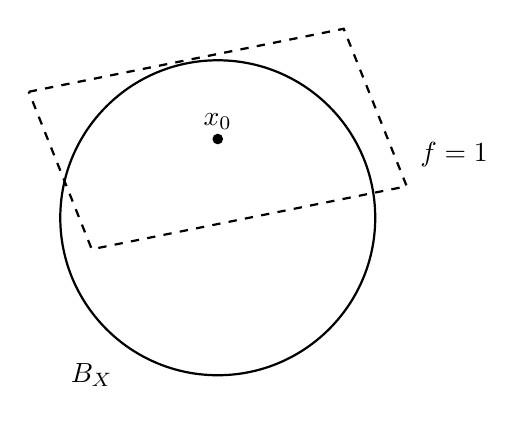
\begin{tikzpicture}[scale=2]

    % Draw the ball B_X (as a circle, no shading)
    \draw[thick] (0,0) circle (1);  % The ball B_X
    
    % Label B_X
    \node at (-0.8,-1) {$B_X$};

    % Draw the tangent plane at an angle (as a parallelogram)
    \draw[thick, dashed] (-1.2,0.8) -- (0.8,1.2) -- (1.2,0.2) -- (-0.8,-0.2) -- cycle;  % Tangent plane (parallelogram)
    
    % Mark point x_0 on the ball and the tangent plane
    \filldraw[black] (0,0.5) circle (0.03) node[anchor=south] {$x_0$};

    % Label the tangent plane f=1
    \node at (1.5,0.4) {$f = 1$};
\end{tikzpicture}
\end{center}

\subsection{Bidual}%
\label{sub:bidual}

Let $X$ be a normed space. Then $X^{\ast\ast} = (X^\ast)^\ast$ is the \emph{bidual}\index{bidual} or \emph{second dual} of $X$.

For $x \in X$, define $\hat x$ on $X^\ast$ by $f \mapsto f(x)$, i.e. evaluation at $x$.

Then $\hat x$ is linear, and
\[
|\hat x(f)| = |f(x)| \leq \|f\| \|x\|,
\]
for all $f \in X^\ast$. So $\hat x \in X^{\ast\ast}$, and $\|\hat x\| \leq \|x\|$. The map $x \mapsto \hat x$ is the \emph{canonical embedding} of $X$ into $X^{\ast\ast}$.

\begin{theorem}
	The canonical embedding is an isometric isomorphism of $X$ into $X^{\ast\ast}$.
\end{theorem}

\begin{proofbox}
	Linearity: note
	\begin{align*}
		\widehat{\lambda x + \mu y}(f) &= f(\lambda x + \mu y) = \lambda f(x) + \mu f(y) \\
					       &= (\lambda \hat x + \mu \hat y)(f).
	\end{align*}
	Isometric: for $x \in X$,
	\[
		\|\hat x\| = \sup\{|f(x)| \mid f \in B_{X^\ast} \} = \|x\|,
	\]
	by Hahn-Banach.
\end{proofbox}

\begin{remark}
	\begin{enumerate}
		\item[]
		\item Note that
			\[
			\langle f, \hat x \rangle = \langle x, f \rangle,
			\]
			for $x \in X$, $f \in X^\ast$.
		\item $\hat X = \{\hat x \mid x \in X \} \cong X$. Therefore,
			\[
				\hat X \text{ is closed in } X^{\ast\ast} \iff X \text{ is complete}.
			\]
		\item In general, the closure in $X^{\ast\ast}$ of $\hat X$ is a Banach space containing an isometric copy of $X$ as a dense subspace.
	\end{enumerate}
\end{remark}

\begin{definition}
	A normed space $X$ is \emph{reflexive}\index{reflexive} if the canonical embedding $X \to X^{\ast\ast}$ is surjective.
\end{definition}

\begin{exbox}
	\begin{enumerate}
	\item Any finite-dimensional space is reflexive.
	\item $\ell_p$ for $1 < p < \infty$ is reflexive.
	\item 	Any Hilbert space is reflexive.
	\item $L_p(\mu)$ for $1 < p < \infty$ is reflexive.
	\item $c_0, \ell_1, \ell_\infty, L_1([0, 1])$ are not reflexive.
\end{enumerate}
\end{exbox}

\begin{remark}
	If $X$ is reflexive, then $X$ is a Banach space, and $X \cong X^{\ast\ast}$.

	However, there exists a Banach space $X$ such that $X \cong X^{\ast\ast}$, but $X$ is not reflexive. So even though $\ell_p^{\ast\ast} \cong \ell_q^\ast \cong \ell_p$, this is not enough to show $\ell_p$ is reflexive.
\end{remark}


% lecture 3

\subsection{Dual Operators}%
\label{sub:dual_op}

Let $X, Y$ be normed spaces. Then,
\[
	\mathcal{B}(X, Y) = \{T : X \to Y \mid T \text{ linear, bounded}\}.
\]
Recall that $\mathcal{B}(X, Y)$ is a normed space with the operator norm:
\[
	\|T\| = \sup \{ \|Tx\| \mid x \in B_X\}.
\]
If $Y$ is complete, then $\mathcal{B}(X, Y)$ is complete.

For $T \in \mathcal{B}(X, Y)$, its \emph{dual operator}\index{dual operator} $T^\ast : Y^\ast \to X^\ast$ is given by
\[
T^\ast(g) = g \circ T.
\]
This is well-defined, and in the bracket notation
\[
\langle x, T^\ast g \rangle = \langle T x, g \rangle.
\]
It is easy to see that $T^\ast$ is linear, and moreover it is bounded. Note
\begin{align*}
	\|T^\ast\| &= \sup_{g \in B_{Y^\ast}} \|T^\ast g\| = \sup_{g \in B_{Y^\ast}} \sup_{x \in B_X} | \langle x, T^\ast g \rangle| = \sup_{x \in B_X} \sup_{g \in B_{Y^\ast}} | \langle Tx, g \rangle | \\
		   &\overset{HB}= \sup_{x \in B_x} \|Tx\| = \|T\|.
\end{align*}

\begin{remark}
	If $X, Y$ are Hilbert spaces, and we identify $X, Y$ with $X^\ast, Y^\ast$ respectively, then $T^\ast$ becomes the \emph{adjoint}\index{adjoint} of $T$.
\end{remark}

\begin{exbox}
	If $1 \leq p < \infty$, and $R : \ell_p \to \ell_p$ is the right-shift, then $R^\ast : \ell_q \to \ell_q$ is the left-shift.
\end{exbox}

We have the following properties:
\begin{itemize}
	\item $(\id_X)^\ast = \id_{X^\ast}$.
	\item $(\lambda S + \mu T)^\ast = \lambda S^\ast + \mu T^\ast$.
	\item $(ST)^\ast = T^\ast S^\ast$.
	\item $T \mapsto T^\ast : \mathcal{B}(X, Y) \to \mathcal{B}(Y^\ast, X^\ast)$ is an into isometric isomorphism.
	\item The following diagram commutes:
		\[
		\begin{tikzcd}
			X \arrow[r, "T"] \arrow[d] & Y \arrow[d] \\
			X^{\ast\ast} \arrow[r, "T^{\ast\ast}"] & Y^{\ast\ast}
		\end{tikzcd}
		\]
		In other words $\widehat{T x} = T^{\ast\ast} \hat x$, for all $x \in X$.
\end{itemize}

Indeed, for all $x \in X$, $g \in Y^\ast$,
\begin{align*}
	\braket{g, T^{\ast\ast} \hat x} &= \langle T^{\ast} g, \hat x \rangle = \langle x, T^{\ast} g\rangle \\
					       &= \langle Tx, g\rangle = \langle g, \widehat{Tx}\rangle.
\end{align*}

\subsection{Quotient spaces}%
\label{sub:qp}

Let $X$ be a NVS and $Y$ be a closed subspace. Then $X/Y$ is a normed space in the \emph{quotient norm}\index{quotient norm}:
\[
	\|x + Y\| = \inf\{ \|x + y\| \mid y \in Y\} = d(x, Y).
\]
Here closed is important, so that $\|x + Y\| = 0 \implies x \in Y$.

The quotient map $q : X \to X/Y$ is linear, surjective and bounded with $\|q\| = 1$, since for $x \in X$ 
\[
\|q(x)\| \leq \|x\|.
\]
Letting $D_X$ be the open unit ball of $X$, we can show $q(D_X) = D_{X/Y}$. Indeed if $x \in D_X$, then $\|q(x)\| \leq \|x\| < 1$. If $\|x + Y\| < 1$, then there exists $y \in Y$ with $\|x + y\| < 1$. So $x + y \in D_X$ and $q(x + y) = x + Y$.

So $\|q\| = 1$, unless $Y = X$. Also, $q$ is an open map.

Assume $T : X \to Z$ is a bounded linear map, and $Y \subseteq \ker T$. Then there exists a unique map $\tilde T : X/Y \to Z$ such that the following diagram commutes:
\[
\begin{tikzcd}
	X \arrow[rr, "T"] \arrow[dr, "q"] & & Z \\
					  & X/Y \arrow[ur, "\tilde T"] &
\end{tikzcd}
\]
Moreover, $\tilde T$ is linear and bounded, and $\|\tilde T\| = \|T\|$, since
\[
\tilde T(D_{X/Y}) = \tilde T(q(D_X)) = T(D_X).
\]

\begin{theorem}
	Let $X$ be a normed space. If $X^\ast$ is separable, then so is $X$.
\end{theorem}

\begin{remark}
	The converse is false in general, by taking $X = \ell_1$, then $X^\ast = \ell_\infty$.
\end{remark}

\begin{proofbox}
	Since $X^\ast$ is separable, so is $S_{X^\ast}$. Let $(f_n)$ be a dense sequence in $S_{X^\ast}$. For all $n \in \mathbb{N}$, choose $x_n \in B_X$ such that $|f_n(x_n)| > 1/2$.

	Set $Y = \overline{\spn}\{x_n \mid n \in \mathbb{N}\}$, the closed linear span of $x_n$ Then we claim $Y = X$.

	Assume not. Then we first find $f \in S_{X^\ast}$ such that $f|_Y = 0$. Since $X/Y \neq \{0\}$, we have $(X/Y)^\ast \neq \{0\}$, by Hahn-Banach. Choose any $g \in S_{(X/Y)^\ast}$.

	Let $f = g \circ q$. Then $\|f\| = \|g\| = 1$, so $f \in S_{X^\ast}$, and $f|_Y = 0$.

	Choose $n \in \mathbb{N}$ such that $\|f - f_n\| < 1/10$. Now,
	\begin{align*}
		\frac{1}{2} &< |f_n(x_n)| = |(f_n - f)(x_n)| \leq \|f_n - f\| \cdot \|x_n\| < \frac{1}{10},
	\end{align*}
	a contradiction.
\end{proofbox}

\begin{theorem}
	Let $X$ be a separable normed space. Then $X$ is isometrically isomorphic to a subspace of $\ell_\infty$.
\end{theorem}

Consider a map $T : X \to \ell_\infty$. The $n$'th coordinate is then a linear function of $x$, that is bounded, hence is a functional. So we can think of
\[
Tx = (f_n(x)).
\]
We also want $\|Tx\|_\infty = \|x\|$, which we can do by choosing a norming functional (or an appropriate approximate).

\begin{proofbox}
	Let $(x_n)$ be a dense sequence in $X$. For each $n \in \mathbb{N}$, choose $f_n \in S_{X^\ast}$ such that $f_n(x_n) = \|x_n\|$.

	Define $T : X \to \ell_\infty$ by
	\[
		T(x) = (f_1(x), f_2(x), \ldots).
	\]
	Note that $|f_n(x)| \leq \|x\|$, so $T$ is well-defined, linear and bounded with norm at most 1.

	But for each $n$,
	\[
	\|Tx_n\|_{\infty} \geq |f_n(x_n)| = \|x_n\|,
	\]
	so $\|Tx_n\|_{\infty} = \|x_n\|$. Since $(x_n)$ is dense, and continuity of $T$, we have $\|Tx\| = \|x\|$ for all $x \in X$.
\end{proofbox}

\begin{remark}
	We say that $\ell_\infty$ is \emph{isometrically universal}\index{isometrically universal} for the class $\mathcal{SB}$ of all separable Banach spaces.
\end{remark}

\begin{theorem}[Vector-valued Liouville's Theorem]
	Let $X$ be a complex Banach space, and $f : \mathbb{C} \to X$ bounded and holomorphic. Then $f$ is constant.
\end{theorem}

\begin{proofbox}
	Since $f$ is bounded, there is $M \in \mathbb{R}$ such that for all $z \in \mathbb{C}$, $\|f(z)\| \leq M$.

	$f$ is holomorphic means that
	\[
	\lim_{w \to z} \frac{f(w) - f(z)}{w - z}
	\]
	exists, and is denoted by $f'(z)$, for all $z \in \mathbb{C}$.

	Fix $\phi \in X^\ast$. Since $\phi$ is linear and continuous,
	\[
	\lim_{w \to z} \frac{\phi(f(w)) - \phi(f(z))}{w - z} = \phi \left( \lim_{w \to z} \frac{f(w) - f(z)}{w - z} \right).
	\]
	So $\phi \circ f : \mathbb{C} \to \mathbb{C}$ is entire.

	Also, for all $z \in \mathbb{C}$, $|\phi(f(z))| \leq \|\phi\| \cdot \|f(z)\| \leq M \dot \|\phi\|$. So by Liouville, $\phi \circ f$ is constant, hence $\phi(f(z)) =\phi(f(0))$ for all $z \in \mathbb{C}$.

	Fix $z \in \mathbb{C}$. Since $X^\ast$ separates the points of $X$, $f(z) = f(0)$.
\end{proofbox}

% lecture 4

\subsection{Locally Convex Spaces}%
\label{sub:lcs}

\begin{definition}
	A \emph{locally convex space}\index{locally convex space} (LCS) is a pair $(X, \mathcal{P})$ where $X$ is a real or complex vector space, and $\mathcal{P}$ is a family of seminorms on $X$ such that $\mathcal{P}$ separates the points of $X$, i.e. for all $x \in X \setminus \{0\}$, there exists $p \in \mathcal{P}$ with $p(x) \neq 0$.
\end{definition}

The family $\mathcal{P}$ defines a topology on $X$ as follows: $U \subseteq X$ is open if and only if, for all $x \in U$, there are seminorms $p_1, \ldots, p_n \in \mathcal{P}$ and $\eps > 0$ such that
\[
	\{y \in X \mid p_k(y - x) < \eps \text{ for } k = 1, \ldots, n\} \subseteq U.
\]
So the open balls form a base of the topology.

\begin{remark}
	\begin{enumerate}[1.]
		\item[]
		\item Addition and scalar multiplication are continuous.
		\item This is Hausdorff, as $\mathcal{P}$ separates the points.
		\item $x_n \to x$ in $X$ if and only if $p(x_n - x) \to 0$ for all $p \in \mathcal{P}$.
		\item Let $Y$ be a subspace of $X$. Let $\mathcal{P}_Y = \{p|_Y \mid p \in \mathcal{P}\}$. Then $(Y, \mathcal{P}_Y)$ is a LCS, and the topology of $(Y, \mathcal{P}_Y)$ is the subspace topology induced by the topology of the LCS $(X, \mathcal{P})$.
		\item Let $\mathcal{P}, \mathcal{Q}$ be two families ofseminorms on $X$, both separating points of $X$. Say $\mathcal{P}, \mathcal{Q}$ are \emph{equivalent}\index{equivalent seminorms}, and we write $P \sim Q$, if they generate the same topology on $X$.

			The topology of a LCS $(X, \mathcal{P})$ is metrizable if and only if there is a countable $Q \sim P$.
	\end{enumerate}
\end{remark}

\begin{definition}
	A \emph{Fr\'echet space}\index{Fr\'echet space} is a complete metrizable LCS.
\end{definition}

\begin{exbox}
	\begin{enumerate}
		\item A normed space $(X, \|\cdot\|)$ is a LCS with $\mathcal{P} = \{\|\cdot\|\}$.
		\item Let $U \subseteq \mathbb{C}$ be a non-empty open set, and
			\[
				\mathcal{O}(U) = \{ f : U \to \mathbb{C} \mid f \text{ holomorphic}\}.
			\]
			For $K \subseteq U$, $K$ compact, let
			\[
			p_K(f) = \sup_{z \in K} |f(z)|,
			\]
			for $f \in \mathcal{O}(U)$. Let $\mathcal{P} = \{p_K \mid K \subseteq U, K \text{ compact}\}$. Then $(\mathcal{O}(U), \mathcal{P})$ is a LCS. The topology is the topology of local uniform convergence.

			Note that there exists $(K_n)$ of compact subsets of $U$ such that $K_n \subseteq \mathrm{int} K_{n+1}$ for all $n$, and $\bigcup K_n = U$, and
			\[
				\{ p_{K_n} \mid n \in \mathbb{N}\} \sim \mathcal{P}.
			\]
			So $(\mathcal{O}(U), \mathcal{P})$ is metrizable, and in fact a Fr\'echet space. This topology is not normable, i.e. there is no norm on $\mathcal{O}(U)$ inducing the same topology (can use Montel's theorem).
		\item Take $d \in \mathbb{N}$, and $\Omega \subseteq \mathbb{R}^d$ non-empty and open. Take
			\[
				C^\infty(\Omega) = \{f : \Omega \to \mathbb{R} \mid f \text{ infinitely differentiable}\}.
			\]
			For a multiindex $\alpha = (\alpha_1, \ldots, \alpha_n)$, we have a differential operator $D^\alpha$ given by
			\[
			D^\alpha f = \left( \frac{\partial}{\partial x^1} \right)^{\alpha_1} \cdots \left( \frac{\partial}{\partial x^n} \right)^{\alpha_n}.
			\]
			For $\alpha \in (\mathbb{Z}_{\geq 0})^d$, $K \subseteq \Omega$ compact, define
			\[
				p_{K, \alpha}(f) = \sup\{ |(D^\alpha)f(x)| \mid x \in K\}.
			\]
			Let $\mathcal{P} = \{p_{K, \alpha} \mid \alpha \text{ multiindex}, K \text{ compact}\}$. Then $(C^\infty(\Omega), \mathcal{P})$ is a LCS, which is a Fr\'echet space that is not normable.
	\end{enumerate}
	
\end{exbox}

\begin{lemma}
	Let $(X, \mathcal{P})$ and $(Y, \mathcal{Q})$ be LCS, and $T : X \to Y$ a linear map. Then the following are equivalent:
	\begin{enumerate}[\normalfont(i)]
		\item $T$ is continuous.
		\item $T$ is continuous at $0$.
		\item For all $q \in \mathcal{Q}$, there are seminorms $p_1, \ldots, p_n \in \mathcal{P}$ and $C \geq 0$ such that for all $x$,
			\[
			q(Tx) \leq C \max_{1 \leq k \leq n} p_k(x).
			\]
	\end{enumerate}
\end{lemma}

\begin{proofbox}
	It is easy to see (i) $\iff$ (ii), since translations are a homeomorphism.

	We show (ii) $\implies$ (iii). Let $q \in \mathcal{Q}$, and $V = \{y \in Y \mid q(y) < 1\}$ a neighbourhood of $0$ in $Y$. As $T$ is continuous at $0$, there exists a neighbourhood of 0 in $X$ such that $T(U) \subseteq V$. Without loss of generality,
	\[
		U = \{x \in X \mid p_k(X) \leq \eps, k = 1, \ldots, n\}
	\]
	for some $n \in \mathbb{N}$, and $p_1, \ldots, p_n \in \mathcal{P}$, $\eps > 0$.

	Let $p(x) = \max_{1 \leq k \leq n} p_k(x)$. We show that $q(Tx) \leq \frac{1}{\eps} p(x)$ for all $x \in X$. Let $x \in X$. If $p(x) \neq 0$, then
	\[
	p \left( \frac{\eps x}{p(x)} \right) = \eps,
	\]
	so
	\[
	\frac{\eps x}{p(x)} \in U \implies T \left( \frac{\eps x}{p(x)} \right) \in V.
	\]
	Therefore,
	\[
	q \left( T \left( \frac{\eps x}{ p(x)} \right) \right) < 1 \implies q(Tx) \leq \frac{1}{\eps} p(x).
	\]
	If $p(x) = 0$, then $\lambda x \in U$ for all scalars $\lambda$, hence $q(T(\lambda x)) < 1$ for all $\lambda$. So $q(Tx) = 0$.

	Now we show (iii) $\implies$ (ii). Let $V$ be an open neighbourhood of $0$ in $Y$. We seek a neighbourhood $U$ of $0$ in $X$ such that $T(U) \subseteq V$. Without loss of generality,
	\[
		V = \{y \in Y \mid q_k(y) < \eps, k = 1, \ldots, m\}.
	\]
	For each $k= 1, \ldots, m$, there exist seminorms $p_{k,1}, \ldots, p_{k,n_k} \in \mathcal{P}$ and $C_k > 0$ such that for all $x \in X$,
	\[
	q_k(Tx) \leq C_k \max_{1 \leq j \leq n_k} p_{k, j}(x).
	\]
	Then,
	\[
		U = \{x \in X \mid p_{k, j}(x) \leq \frac{\eps}{C_k}, k = 1, \ldots, m, j =1, \ldots, n_k \}
	\]
	is a neighbourhood of $0$ in $X$, and for each $x \in U$,
	\[
	q_k(Tx) \leq C_k \max_{1 \leq j \leq n_k} p_{k, j}(x) < \eps
	\]
	for each $k = 1, \ldots, m$, so $Tx \in V$,
\end{proofbox}

\begin{definition}
	The \emph{dual space}\index{dual space of LCS} of a LCS $(X, \mathcal{P})$ is the space $X^\ast$ of all linear functional of $X$ which are continuous with respect to the topology of $X$.
\end{definition}

\begin{lemma}
	Let $f$ be a linear functional on a LCS $X$. Then,
	\[
		f \in X^\ast \iff \ker f\text { is closed}.
	\]
\end{lemma}

\begin{proofbox}
	One way is obvious: if $f$ is continuous, then $\ker f = f^{-1}(\{0\})$ must be closed.

	Now consider the other direction. We can assume without loss of generality that $f \neq 0$. Fix $x_0 \in X \setminus \ker f$. Since $\ker f$ is closed, there is a neighbourhood $U$ of $0$ in $X$, such that $x_0 + U$ is disjoint from $\ker f$.

	Without loss of generality,
	\[
		U = \{x \in X \mid p_k(x) < \eps, k = 1, \ldots, n\}
	\]
	for seminorms $p_1, \ldots, p_n \in \mathcal{P}$.

	Note that $U$ is convex and \emph{balanced}\index{balanced} (if $x \in U$, $|\lambda| = 1$ a scalar then $\lambda x \in U$) since $p_i$ are seminorms.

	As $f$ is linear, $f(U)$ is also convex and balanced. Hence it is an interval or a disc.

	But since $-f(x_0) \not \in f(U)$, otherwise $0 \in f(x_0 + U)$, $f(U)$ is bounded. Hence
	\[
		f(U) \subseteq \{\lambda \text{ a scalar} \mid |\lambda| < M\}.
	\]
	Hence for any $\delta > 0$,
	\[
		f \left( \frac{\delta}{M} U\right) \subseteq \{\lambda \text{ a scalar} \mid |\lambda| < \delta\},
	\]
	and $\frac{\delta}{M} U$ is a neighbourhood of $0$. Thus $f$ is continuous at $0$.
\end{proofbox}

% lecture 5

\begin{theorem}[Hahn-Banach]
	Let $(X, \mathcal{P})$ be a LCS.
	\begin{enumerate}[\normalfont(i)]
		\item If $Y$ is a subspace of $X$ and $g \in Y^\ast$, then there exists $f \in X^\ast$ such that $f|_Y = g$.
		\item If $Y$ is a closed subspace of $X$ and $x_0 \in X \setminus Y$, then there exists $f \in X^\ast$ such that $f|_Y = 0$, and $f(x_0) \neq 0$.
	\end{enumerate}
\end{theorem}

\begin{proofbox}
	

	(i) By lemma 1.1, there exists $p_1, \ldots, p_n \in \mathcal{P}$, and $C \geq 0$ such that for all $y \in Y$,
	\[
	|g(y)| \leq C \max_{1 \leq k \leq n} p_k(y).
	\]
	Define $p : X \to \mathbb{R}$ by
	\[
	p(x) = C \max_{1 \leq k \leq n} p_k(x).
	\]
	Then $p$ is a seminorm on $X$, and on $Y$ $|g(y)| \leq p(y)$ for all $y \in Y$.

	By Hahn-Banach on seminorms, there exists a linear functional $f$ on $X$ such that $f|_Y = g$ and for all $x \in X$, $|f(x)| \leq p(x)$. Lemma 1.1 gives us that $f$ is continuous.

	(ii) Let $Z = \spn(Y \cup \{x_0\})$. Define a linear functional $g$ on $Z$ by
	\[
	g(y + \lambda x_0) = \lambda
	\]
	for $y \in Y$, $\lambda$ a scalar. Notice that $\ker g = Y$ is closed by supposition, so $g$ is continuous, i.e. $g \in Z^\ast$. Then applying (i), we find $f \in X^\ast$ satisfying $f|_Z = g$, so in particular $f|_Y = 0$ and $f(x_0) = g(x_0) = 1$.
\end{proofbox}

\begin{remark}
	$X^\ast$ separates the points of $X$: given $x \neq y$, apply (ii) to $Y = \{0\}$, and $x_0 = x - y$.
\end{remark}

\newpage

\section{Dual Spaces of \texorpdfstring{$L_p(\mu)$}{Lp(mu)} and \texorpdfstring{$C(K)$}{C(K)}}%
\label{sec:ds}

Let $(\Omega, \mathcal{F}, \mu)$ be a measure space, and let $1 \leq p < \infty$. Recall
\[
	L_p(\mu) = \left\{f : \Omega \to \text{scalars} \biggm| f \text{ measurable}, \int_{\Omega} |f|^p \diff \mu < \infty\right\}.
\]
This is a normed space in the $L_p$-norm,
\[
\|f\|_p = \left( \int_{\Omega} |f|^p \diff \mu \right)^{1/p}.
\]
We identify functions $f, g$ if $f = g$ almost everywhere. If $p = \infty$, then
\[
	L_\infty(\mu) = \{f : \Omega \to \text{scalars} \mid f \text{ measurable, essentially bounded}\}.
\]
Essentially bounded means $f$ is bounded, up to a null set. This is a normed space in the $L_\infty$ norm:
\[
	\|f\|_\infty = \mathrm{ess} \sup |f| = \inf \{ \sup_{\Omega \setminus N} |f| \mid N \in \mathcal{F}, \mu(N) = 0\}.
\]
The infimum can be attained by taking $N_i$ that limit to the infimum, and then taking their union.

\begin{remark}
	If $\|\cdot\|$ is a seminorm on a vector space $X$, then
	\[
		N = \{x \in X \mid \|x\| = 0\}
	\]
	is a subspace of $X$, and $\|x + N\| = \|x\|$ defines a norm on the quotient.
\end{remark}

We will not think like this for $L_p$.

\begin{theorem}
	$L_p(\mu)$ is a Banach space for $1 \leq p \leq \infty$.
\end{theorem}

Our aim is to describe $L_p(\mu)^\ast$.

\subsection{Complex Measures}%
\label{sub:comp_m}

Let $\Omega$ be a set, and $\mathcal{F}$ be a $\sigma$-algebra on $\Omega$. A \emph{complex measure}\index{complex measure} on $\mathcal{F}$ is a countably additive set function $\nu : \mathcal{F} \to \mathbb{C}$.

The \emph{total variation measure}\index{total variation measure} of $\nu$, denoted by $|\nu|$, is defined as follows: for $A \in \mathcal{F}$,
\[
	|\nu|(A) = \sup \left\{  \sum_{k = 1}^n |\nu(A_k)| \biggm| A = \bigcup_{k = 1}^n A_k \text{ is a measurable partition of } A \right\}.
\]
Then $|\nu| : \mathcal{F} \to [0, \infty]$ is a positive measure, and is the smallest measure such that for all $A \in \mathcal{F}$,
\[
|\nu(A)| \leq |\nu|(A).
\]
In other words, if $\mu$ is a positive measure on $\mathcal{F}$ and for all $A \in \mathcal{F}$, $|\nu(A)| \leq \mu(A)$, then $|\nu|(A) \leq \mu(A)$.

The \emph{total variation}\index{total variation} of $\nu$ is
\[
\|\nu\|_1 = |\nu|(\Omega).
\]
As currently defined this could be infinite, but we will see that this is always finite.

$\nu$ satisfies the two continuity conditions:
\begin{itemize}
	\item If $A_n \subseteq A_{n+1}$, then
		\[
		\nu\left( \bigcup_{n = 1}^\infty A_n \right) = \lim_{n \to \infty} \nu(A_n).
		\]
	\item If $A_n \supseteq A_{n+1}$, then
		\[
		\nu\left( \bigcap_{n = 1}^\infty A_n \right) = \lim_{n \to \infty} \nu(A_n).
		\]
\end{itemize}

\emph{Signed measures}\index{signed measures} are complex measures that take real values, i.e. countably additive set functions $\mathcal{F} \to \mathbb{R}$.

\begin{theorem}
	Let $(\Omega, \mathcal{F})$ be as before, and $\nu$ a signed measure on $\mathcal{F}$.

	Then there exists a measurable partition $\Omega = P \cup N$ of $\Omega$ such that for all $A \in \mathcal{F}$ and $A \subseteq P$, then $\nu(A) \geq 0$, and if $A \subseteq N$ then $\nu(A) \leq 0$.
\end{theorem}

\begin{remark}
	\begin{enumerate}
		\item[]
		\item $\Omega = P \cup N$ is the \emph{Hahn decomposition}\index{Hahn decomposition} of $\Omega$ (or of $\nu$).
		\item Let $\nu^+(A) = \nu(A \cap P)$ and $\nu^-(A) = - \nu(A \cap N)$ for $A \in \mathcal{F}$.

			Then $\nu^+$, $\nu^-$ are finite positive measures such that $\nu = \nu^+ - \nu^-$, and $|\nu| = \nu^+ + \nu^-$.

			These properties determine $\nu^+$ and $\nu^-$ uniquely. This decomposition $\nu = \nu^+ - \nu^-$ is the \emph{Jordan decomposition}\index{Jordan decomposition} of $\nu$.
		\item Let $\nu$ be a complex measure. Then $\Re (\nu)$ and $\Im(\nu)$ are signed measures with Jordan decompositions $\nu_1 - \nu_2$ and $\nu_3 - \nu_4$. Then,
			\[
			\nu = \nu_1 - \nu_2 + i(\nu_3 - \nu_4).
			\]
			This is the \emph{Jordan decomposition} of $\nu$. Note that $\nu_k \leq |\nu|$, and
			\[
			|\nu| \leq \nu_1 + \nu_2 + \nu_3 + \nu_4.
			\]
			So $|\nu|$ is a finite measure since $\nu_1, \nu_2, \nu_3, \nu_4$ are all finite, so $\|\nu\|_1 < \infty$.
		\item Suppose the signed measure $\nu$ has Hahn decomposition $\Omega = P \cup N$ and Jordan decomposition $\nu^+ - \nu^-$. For $A, B \in \mathcal{F}$ with $B \subseteq A$,
			\[
			\nu^+(A) \geq \nu^+(B) \geq \nu(B),
			\]
			and $\nu^+(A) = \nu(B)$ if $B = P \cap A$. So,
			\[
				\nu^+(A) = \sup \{ \nu(B) \mid B \in \mathcal{F}, B \subseteq A\}.
			\]
	\end{enumerate}
\end{remark}

\begin{proofbox}
	This is a non-examinable sketch.

	Define
	\[
		\nu^+(A) = \sup \{\nu(B) \mid B \in \mathcal{F}, B \subseteq A\} \geq 0,
	\]
	since we may always take $B = \emptyset$. It is clear that $\nu^+(\emptyset) = 0$, and $\nu^+$ is finitely additive.

	The main claim is that $\nu^+(\Omega) < \infty$. Assume not. Inductively construct $(A_n), (B_n)$ in $\mathcal{F}$ such that $A_0 = \Omega$, and if $\nu^+(A_{n-1}) = \infty$, pick $B_n \subseteq A_{n-1}$, with $\nu(B_n) > n$.

	Then pick either $A_n = B_n$ or $A_{n-1} \setminus B_n$ such that $\nu^+(A_n) = \infty$.

	We can then use continuity of $\nu$ to get a contradiction, by condition on whether $A_n = B_n$ eventually, or $A_n = A_{n-1} \setminus B_n$ infinitely often.

	The next claim is that the supremum is achieved, so there exists $P \in \mathcal{F}$ such that
	\[
		\nu^+(\Omega) = \nu(P).
	\]
	Choose $A_n \in \mathcal{F}$, with $\nu(A_n) > \nu^+(\Omega) - 2^{-n}$, and we can check
	\[
	P = \bigcup_m \bigcap_{n \geq m} A_n
	\]
	works. Then letting $N = \Omega \setminus P$, we can check this works as a partition.
\end{proofbox}

% lecture 6

\begin{definition}
	Fix a measure space $(\Omega, \mathcal{F}, \mu)$. A complex measure $\nu : \mathcal{F} \to \mathbb{C}$ is \emph{absolutely continuous}\index{absolute continuous} with respect to $\mu$, written $\nu \ll \mu$, if for all $A \in \mathcal{F}$,
	\[
	\mu(A) = 0 \implies \nu(A) = 0.
	\]
\end{definition}

\begin{remark}
	\begin{enumerate}
		\item[]
		\item If $\nu \ll \mu$, then $|\nu| \ll \mu$. It follows that if $\nu = \nu_1 - \nu_2 + i \nu_3 - i \nu_4$ is the Jordan decomposition of $\nu_1$, then 
			\[
			\nu \ll \mu \iff \nu_k \ll \mu
			\]
			for all $k$ (note that $\nu_1, \nu_2$ are non-zero on different subsets of $\mathcal{F}$).
		\item If $\nu \ll \mu$, then for all $\eps > 0$, there exists $\delta > 0$ such that for any $A \in \mathcal{F}$,
			\[
			\mu(A) < \delta \implies |\nu(A)| < \eps.
			\]
	\end{enumerate}
\end{remark}

\begin{exbox}
	If $f \in L_1(\mu)$, then
	\[
	\nu(A) = \int_A f \diff \mu,
	\]
	for $A \in \mathcal{F}$, defines a complex measure on $\mathcal{F}$ (by dominated convergence), and $\nu \ll \mu$.
\end{exbox}

\begin{definition}
	A set $A \in \mathcal{F}$ is $\sigma$-finite with respect to $\mu$ if there exists $(A_n)$ in $\mathcal{F}$ such that
	\[
	A = \bigcup_{n \in \mathbb{N}} A_n, \qquad \mu(A_n) < \infty.
	\]
	We say that $\mu$ is $\sigma$-finite if $\Omega$ is a $\sigma$-finite set (so every $A \in \mathcal{F}$ is $\sigma$-finite).
\end{definition}

\begin{theorem}[Radon-Nikodym Theorem]
	Let $(\Omega, \mathcal{F}, \mu)$ be a $\sigma$-finite measure and $\nu : \mathcal{F} \to \mathbb{C}$ be a complex measure such that $\nu \ll \mu$.

	Then there exists a unique $f \in L_1(\mu)$ such that
	\[
	\nu(A) = \int_A f \diff \mu,
	\]
	for all $A \in \mathcal{F}$. Moreover $f$ takes values in $\mathbb{C}$ or $\mathbb{R}$ or $\mathbb{R}^+$ depending on whether $\nu$ is a complex/signed/positive measure.
\end{theorem}

\begin{proofbox}
	This is a non-examinable sketch.

	First we show uniqueness. This follows as if $f \in L_1(\mu)$ and $\int_A f \diff \mu = 0$, then $f = 0$ almost everywhere.

	For existence, first assume $\nu$ is a finite positive measure, by taking the Jordan decomposition.

	We can also assume $\mu$ is finite: for each partition $A_i$ we have function $f_i$, which we can glue together; this extends by monotone convergence, since we first assumed $\nu$ is finite and positive.

	Now let
	\[
		\mathcal{H} = \left\{h : \Omega \to \mathbb{R}^+ \biggm| \int_A h \diff \mu \leq \nu(A) \text{ for all } A \in \mathcal{F}\right\}.
	\]
	Note $0 \in \mathcal{H}$, $h_1, h_2 \in \mathcal{H} \implies h_1  \vee H_2 \in \mathcal{H}$, and if $h_n \in \mathcal{H}$, then $h_n \uparrow h \implies h \in \mathcal{H}$. Let
	\[
		\mathcal{L} = \sup \left\{ \int_{\Omega} h \diff \mu \biggm| h \in \mathcal{H} \right\}.
	\]
	This sup is attained (by monotone convergence). Hence there exists $f \in \mathcal{H}$ which attains $\mathcal{L}$. We show that
	\[
	\int_A f \diff \mu = \nu(A),
	\]
	for all $A \in \mathcal{F}$. The idea is that if there exists $A$ with
	\[
	\int_A f \diff \mu < \nu(A),
	\]
	then $f + \delta \mathbbm{1}_{A}$ should be in $\mathcal{H}$ for some $\delta > 0$, contradicting the maximality. However this doesn't quite work as we may fail the condition for $B \subseteq A$.

	For $n \in \mathbb{N}$, define
	\[
	\nu_n(A) = \nu(A) - \int_A f \diff \mu - \frac{1}{n} \mu(A) = \nu(A) - \int_A \left(f + \frac{1}{n} \right) \diff \mu,
	\]
	for all $A \in \mathcal{F}$. Now $\nu_n$ is a signed measure, so we get a Hahn decomposition
	\[
	\Omega = P_n \cup N_n.
	\]
	Then, $f + \frac{1}{n} \mathbbm{1}_{P_n} \in \mathcal{H}$, so $\mu(P_n) = 0$ to not contradict maximality.

	Let $P = \bigcup P_n$. Then $\mu(P) = 0$, so $\nu(P) = 0$ by absolute continuity.

	Set $N = \bigcap N_n$. Then,
	\begin{align*}
		\nu(A) &= \nu(A \cap N) = \nu_n(A \cap N) + \int_{A \cap N}  f \diff \mu + \frac{1}{n} \mu(A \cap N) \\
		       &\leq \int_A f \diff \mu + \frac{1}{n} \mu(A \cap N).
	\end{align*}
	Then we let $n \to \infty$.
\end{proofbox}

\begin{remark}
	\begin{enumerate}
		\item[]
		\item The proof shows that every complex measure $\nu : \mathcal{F} \to \mathbb{C}$ has a decomposition $\nu = \nu_1 + \nu_2$, where $\nu_1 \ll \mu$ and $\nu_2 \perp \mu$. This is the \emph{Lebesgue decomposition}\index{Lebesgue decomposition} of $\nu$.
		\item The unique $f \in L_1(\mu)$ in the Radon-Nikodym theorem is the \emph{Radon-Nikodym derivative}\index{Radon-Nikodym derivative} of $\nu$ with respect to $\mu$, denoted by $\diff \nu/ \diff \mu$. For measurable $g$, then $g$ is $\nu$-integrable if and only if $g \cdot \diff \nu/ \diff \mu$ is $\mu$-integrable, and
			\[
			\int_{\Omega} g \diff \nu = \int_{\Omega} g \frac{\diff \nu}{\diff \mu} \diff \mu.
			\]
	\end{enumerate}
\end{remark}

\subsection{Duals of \texorpdfstring{$L_p$}{Lp}}%
\label{sub:dlp}

Fix a measure space $(\Omega, \mathcal{F}, \mu)$, and let $1 \leq p < \infty$. Let $q$ be the conjugate index of $p$, and for $g \in L_q = L_q(\mu)$, define $\phi_g$ on $L_p$ by
\[
\phi_g(f) = \int_{\Omega} fg \diff \mu.
\]
By H\"older's, $fg \in L_1$, and
\[
|\phi_g(f)| \leq \|f\|_p \|g\|_q.
\]
So $\phi_g \in L_p^\ast$, and $\|\phi_g\| \leq \|g\|_q$. So $\phi : L_q \to L_p^\ast$ exists, given by $g \mapsto \phi_g$. This is linear and bounded, with $\|\phi\| \leq 1$.

\begin{theorem}
	Let $(\Omega, \mathcal{F}, \mu)$, and $p, q, \phi$ be as above.
	\begin{enumerate}[\normalfont(i)]
		\item If $1 < p < \infty$, then $\phi$ is an isometric isomorphic, so $L_p^\ast \cong L_q$.
		\item If $p = 1$ and $\mu$ is $\sigma$-finite, then $L_1^\ast \cong L_\infty$.
	\end{enumerate}	
\end{theorem}

\begin{proofbox}
	What remains is to check that $\phi$ is isometric and onto. Fix $g \in L_q$. We need to check that $\|\phi_g\| = \|g\|_q$.

	Let $\lambda : \Omega \to \text{scalars}$ be measurable, with $|\lambda| = 1$ and $\lambda \cdot g = |g|$, i.e. let $\lambda = \mathrm{sign}(g)$.

	For $1 < p < \infty$, let $f = \lambda |g|^{q-1}$. Then,
	\[
	\int_{\Omega} |f|^{p} \diff \mu = \int_{\Omega} |g|^{pq - p} \diff \mu = \int_{\Omega} |g|^q \diff \mu < \infty,
	\]
	so $f \in L_p$, and
	\[
	\|f\|_p = \|g\|_q^{q/p} = \|g\|_q^{q-1}.
	\]
	Then notice
	\[
	\phi_g(f) = \int \lambda g |g|^{q-1} \diff \mu = \|g\|_q^{q} = \|f\|_p \cdot \|g\|_q,
	\]
	so $\|\phi_g\| \geq \|g\|_q$.

	For $p = 1$, let $s < \|g\|_\infty$. Then $\mu(\{|g| > s\}) > 0$. Since $\mathcal{F}$ is $\sigma$-finite, there exists measurable $A \subseteq \{|g| > s\}$, such that $0 < \mu(A) < \infty$. Then $f = \lambda \mathbbm{1}_{A} \in L_1$, and $\|f\|_1 = \mu(A)$. Now,
	\[
	\|\phi_g\| \cdot \mu(A) \geq \phi_g(f) = \int_A |g| \diff \mu \geq s \mu(A).
	\]
	So $\|\phi_g\| \geq s$, and so $\|\phi_g\| \geq \|g\|_{\infty}$.

	The hard part is showing $\phi$ is onto. Fix $\psi \in L_p^\ast$. We seek $g \in L_q$ such that $\psi = \phi_g$.

	The idea is as follows: let $\psi(\mathbbm{1}_{A}) = \int_A g \diff \mu$. Then we can define $\nu(A) = \psi(\mathbbm{1}_{A})$ for $A \in \mathcal{F}$, with $\nu \ll \mu$, and apply Radon-Nikodym. But we have to split into cases to make this work.

	First, consider when $\mu$ is finite. For $A \in \mathcal{F}$, $\mathbbm{1}_{A} \in L_p$, so we can define $\nu(A) = \psi(\mathbbm{1}_{A})$. This is a measure, as if $A = \bigcup A_n$ is a measurable partition, then
	\[
	\sum_{n = 1}^N \mathbbm{1}_{A_n} \to \mathbbm{1}_{A}
	\]
	in $L_p$, by DCT. So,
	\[
	\sum_{n=1}^N \nu(A_n) = \psi \left( \sum_{n=1}^N \mathbbm{1}_{A_n} \right) \to \psi(\mathbbm{1}_{A}) = \nu(A).
	\]
	So $\nu$ is a complex/signed measure. If $\mu(A) = 0$, then $\mathbbm{1}_{A} = 0$ almost everywhere, so $\nu(A) = \psi(\mathbbm{1}_{A}) = 0$. Thus $\nu \ll \mu$. Hence by Radon-Nikodym, there exists $g \in L_1(\mu)$ such that
	\[
	\nu(A) = \int_A g \diff \mu,
	\]
% lecture 7
	for all $A \in \mathcal{F}$. We show that $g \in L_q(\mu)$ and $\psi = \phi_g$, i.e.
	\[
	\psi(f) = \int_{\Omega} fg \diff \mu
	\]
	for all $f \in L_p$. We have
	\begin{align*}
		\psi(\mathbbm{1}_{A}) &= \nu(A) = \int_A g \diff \mu = \int_{\Omega} \mathbbm{1}_{A} g \diff \mu,
	\end{align*}
	hence
	\[
	\psi(f) = \int_{\Omega} fg \diff \mu
	\]
	for all simple functions $f$. Given $f \in L_\infty$, there is a sequence $(f_n)$ of simple functions such that $f_n \to f$ in $L_\infty$. Then $f_n g \to f g$ in $L_1$ by dominated convergence, and $f_n \to f$ in $L_p$, as $\mu$ is finite. Thus
	\[
	\psi(f) = \lim_{n \to \infty} \psi(f_n) = \lim_{n \to \infty} \int_{\Omega} f_n g \diff \mu = \int_{\Omega} f g \diff \mu.
	\]
	Next we deduce that $g \in L_q$. Fix a measurable function $\lambda$ such that $|\lambda| = 1$ and $\lambda g = |g|$.

	Split into cases. For $p \neq 1$, let $A_n = \{|g| \leq n\}$. Then $f = \lambda \mathbbm{1}_{A_n} |g|^{q-1} \in L_\infty$, and
	\[
	\int_{A_n} |g|^q \diff \mu = \int_{\Omega} fg \diff qm = \psi(f) \leq \|\psi\| \cdot \|f\| = \|\psi\| \left(\int_{A_n} |g|^q \diff \mu \right)^{1/p},
	\]
	so
	\[
	\left( \int_{A_n} |g|^q \diff \mu \right)^{1/q} \leq \|\psi\|.
	\]
	Let $n \to \infty$, and use monotone convergence to get $g \in L_q$.

	For $p = 1$, fix $s > \|\psi\|$ and let $A = \{|g| > s\}$. Then $f = \lambda \mathbbm{1}_{A} \in L_\infty$, so
	\[
	s \mu(A) = \int_A |g| \diff \mu = \int_{\Omega} 
f g \diff \mu = \psi(f) \leq \|\psi\| \|f\|_1 = \|\psi\| \mu(A).
	\]
	The only way is if $\mu(A) = 0$, so $g \in L_\infty$.

	Hence, $\psi$ and $\phi_g$ are both in $L_p^\ast$, and $\psi = \phi_g$, on $L_\infty$. Since $L_\infty$ is dense in $L_p$, we get $\psi = \phi_g$. 
\end{proofbox}

Before we continue to our next cases when $\mu$ may not be finite, we need a few pieces notation.

Fix $A \in \mathcal{F}$. Then,
\[
	\mathcal{F}_A = \{B \in \mathcal{F} \mid B \subseteq A\}
\]
is a $\sigma$-algebra on $A$. Define $\mu_A = \mu|_{\mathcal{F}_A}$. Then $(A, \mathcal{F}_A, \mu_A)$ is a measure space, with $L_p(\mu_A) \subseteq L_p(\mu)$. Let
\[
\psi_A = \psi|_{L_p(\mu_A)}.
\]
Let's continue.

\begin{proofbox}
	Let $\psi_A = \psi|_{L_p(\mu_A)}$, the restriction onto a subset. Then $\psi_A \in L_p(\mu_A)^\ast$, and $\|\psi_A\| \leq \|\psi\|$.

	Let $A, B \in \mathcal{F}$ with $A \cap B = \emptyset$. In the case $1 < p < \infty$,
	\begin{align*}
		\|\psi_{A \cup B}\| &= \sup \{|\psi_{A \cup B}(h)| \mid h \in L_p(\mu_{A \cup B}), \|h\|_p \leq 1\} \\
				    &= \sup\{|\psi_A(f) + \psi_B(g)| \mid f \in L_p(\mu_A), g \in L_p(\mu_B), \|f\|_p^p + \|g\|_p^p \leq 1\} \\
				    &= \sup\{a |\psi_A(f)| + b |\psi_B(g)| \mid a, b \geq 0, a^p + b^p \leq 1, \\
				    & \qquad \qquad \qquad \qquad \qquad \qquad \qquad \qquad f \in B_{L_p}(\mu_A), g \in B_{L_p}(\mu_B)\} \\
				    &= \sup\{a \|\psi_A\| + b \|\psi_B\| \mid a, b \geq 0, a^p + b^p \leq 1\} \\
				    &= (\|\psi_A\|^q + \|\psi_B\|^q)^{1/q},
	\end{align*}
	since $(\ell_p^2)^\ast = \cong \ell_q^2$.

	The next case is when $\mu$ is $\sigma$-finite. We have a measurable partition $\Omega = \bigcup A_n$ of $\Omega$, with $\mu(A_n) < \infty$ for all $n$. By the first case, there is $g_n \in L_q(\mu_{A_n})$ with
	\[
	\psi_{A_n} = \phi_{g_n}.
	\]
	Define $g$ such that
	\[
	g|_{A_n} = g_n.
	\]
	When $p = 1$, then
	\[
	\|g\|_\infty = \sup_{n} \|g_n\|_\infty = \sup_n \|\psi_{A_n}\| \leq \|\psi\|.
	\]
	So $g \in L_q$. For $p \neq 1$, note
	\[
	\sum_{n = 1}^N \|g_n\|_q^q = \sum_{n = 1}^N \|\psi_{A_n}\|^q = \|\psi_{A_1 \cup \cdots \cup A_N}\|^q \leq \|\psi\|^q.
	\]
	By monotone convergence, $g \in L_q$. In both cases, $g \in L_q$, so $\phi_g \in L_p(\mu)^\ast$, and so we have
	\[
	\psi|_{L_p(\mu_{A_n})} = \psi_{A_n} = \phi_{g_n} = \phi_g |_{L_p(\mu_{A_n})}.
	\]
	Since $\bigcup L_p(\mu_{A_n})$ has dense linear span in $L_p(\mu)$, we find that $\psi = \phi_g$ on $L_p(\mu)$.

	The final case is for general $\mu$, and $1 < p < \infty$. Choose $(f_n)$ in $B_{L_p}$ such that $\|\psi\| = \lim_n |\psi(f_n)|$. For all $k, n$, note that
	\[
	\mu(|f_n| \geq 1/k) \leq k^p \|f_n\|_p^p < \infty,
	\]
	by Markov's inequality. Hence
	\[
		A = \bigcup_{n, k}\{|f_n| \geq 1/k\}
	\]
	is $\sigma$-finite, and for all $n$, $f_n = 0$ on $\Omega \setminus A$. So $\|\psi_A\| = \|\psi\|$. So,
	\[
	\|\psi_A\| = \|\psi\| = (\|\psi_A\|^q + \|\psi_{\Omega \setminus A}\|^q)^{1/q},
	\]
	and hence $\psi_{\Omega\setminus A} = 0$. Hence we are done by case 2.
\end{proofbox}

\begin{corollary}
	For $1 < p < \infty$, $L_p(\mu)$ is reflexive.
\end{corollary}

\begin{proofbox}
	Let $\phi \in L_p^{\ast\ast}$. We seek $f \in L_p$ such that $\phi = \hat f$, i.e.
	\[
	\phi(\psi) = \hat f(\psi) = \psi(f)
	\]
	for all $\psi \in L_p^\ast$, i.e.
	\[
	\phi(\phi_g) = \phi_g(f)
	\]
	for all $g \in L_q$. The map $g \mapsto \phi(\phi_g)$ is in $L_q^\ast$, so by the previous theorem, there exists $f \in L_p$ such that
	\[
	\phi(\phi_g) = \int_{\Omega} g f \diff \mu = \phi_g(f).
	\]
\end{proofbox}

\subsection{\texorpdfstring{$C(K)$}{C(K)} Spaces}%
\label{sub:ck_sp}

Throughout, we assume that $K$ is a compact Hausdorff space. Here we make a distinction on our base field:
\[
	C(K) = \{f : K \to \mathbb{C} \mid f \text{ continuous}\}.
\]
This is a complex Banach space with the $\|\cdot\|_\infty$ norm. We also denote
\[
	C^{\mathbb{R}}(K) = \{f : K \to \mathbb{R} \mid f \text{ continuous}\},
\]
and another important object is
\[
	C^+(K) = \{f : K \to \mathbb{R}^+ \mid f \text{ continuous}\},
\]
which is a subset of $C^{\mathbb{R}}(K)$ (more specifically a cone). Let
\[
	M(K) = C(K)^\ast =  \{ \phi : C(K) \to \mathbb{C} \mid \phi \text{ linear, bounded}\},
\]
and also we define
\[
	M^{\mathbb{R}}(K) = \{\phi \in M(K) \mid \phi(f) \in \mathbb{R} \text{ for all } f \in C^{\mathbb{R}}(K)\}.
\]
We do not define $M^{\mathbb{R}} = (C^{\mathbb{R}})^\ast$, however we will show this is true. Also define
\[
	M^+(K) = \{\phi : C(K) \to \mathbb{C} \mid \phi \text{ linear, for all } f \in C^+(K), \phi(f) \in \mathbb{R}^+\}.
\] 
We do note assume continuity, however we will show any $f \in M^+$ is continuous, so $M^+ \subseteq M^\mathbb{R}$. The members of this set are the \emph{positive linear functionals}\index{positive linear functionals}.

Our aim is to describe $M(K), M^{\mathbb{R}}(K)$. We will show that it is enough to describe $M^+(K)$.

\begin{lemma}
	\begin{enumerate}[\normalfont(i)]
		\item[]
\item For all $\phi \in M(K)$, there is a unique $\phi_1, \phi_2 \in M^{\mathbb{R}}(K)$ such that
	\[
	\phi = \phi_1 + i \phi_2.
	\]
	\item The map $\phi \mapsto \phi|_{C^{\mathbb{R}(K)}}$, from $M^{\mathbb{R}} \to (C^{\mathbb{R}})^\ast$ is an isometric isomorphism.
	\item $M^+(K) \subseteq M^\mathbb{R}(K)$ and
		\[
			M^+(K) = \{ \phi \in M(K) \mid \|\phi\| = \phi(1_K)\}.
		\]
	\item For all $\phi \in M^\mathbb{R}(K)$, there exists a unique $\phi^+, \phi^-$ such that
		\[
			\phi = \phi^+ - \phi^- \qquad \text{and} \qquad \|\phi\| = \|\phi^+\| + \|\phi^-\|.
		\]
\end{enumerate}
\end{lemma}

\begin{proofbox}
	

	(i) Define $\bar \phi : C(K) \to \mathbb{C}$, by
	\[
	\bar \phi(f) = \overline{\phi(\bar f)}.
	\]
	Then $\bar \phi \in M(K)$, and
	\[
	\phi \in M^{\mathbb{R}}(K) \iff \phi = \bar \phi.
	\]
	First we show uniqueness. If $\phi = \phi_1 + i \phi_2$, then $\bar f = \phi_1 - i \phi_2$, so
	\[
	\phi_1 = \frac{\phi + \bar \phi}{2}, \qquad \phi_2 = \frac{\phi - \bar \phi}{2i}.
	\]
	This also shows existence, by defining $\phi_1, \phi_2$ in this way.
% lecture 8

	(ii) Let $\phi \in M^{\mathbb{R}}$, and $\psi = \phi|_{C^{\mathbb{R}}}$. Note that $\psi \in (C^{\mathbb{R}})^{\ast}$, and moreover $\|\psi\| \leq \|\phi\|$.

	First we show this map is isometric. Let $f \in C(K)$, and $\lambda \in \mathbb{C}$ such that $|\lambda| = 1$ and $|\phi(f)| = \lambda \phi(f)$. Then,
	\begin{align*}
		|\phi(f)| &= \lambda \phi(f) = \phi(\lambda f) = \phi(\Re(\lambda f)) + i \underbrace{\phi(\Im(\lambda f))}_{0 \text{ as } \phi \in M^{\mathbb{R}}} \\
			  &= \phi(\Re(\lambda f)) = \psi(\Re(\lambda f)) \leq \|\psi\| \|\Re(\lambda f)\|_\infty \leq \|\psi\| \|f\|_\infty.
	\end{align*}
	So $\|\phi\| \leq \|\psi\|$. To show this map is onto, say we have $\psi \in (C^{\mathbb{R}})^{\ast}$. Then the obvious way to define $\phi$ is
	\[
	\phi(f) = \psi(\Re(f)) + i \psi(\Im(f)),
	\]
	for $f \in C(K)$. Then $\phi \in M(K)$ and $\phi|_{C^{\mathbb{R}}(K)} = \psi$.

	(iii) To show the inclusion, let $\phi \in M^{+}(K)$, and $f \in C^{\mathbb{R}}(K)$ with $-1 \leq f \leq 1$ on $K$. Then $1_K \pm f \geq 0$ on $K$. So,
	\[
	\phi(1_K \pm f) = \phi(1_K) \pm \phi(f) \geq 0.
	\]
	So $\phi(f) \in \mathbb{R}$, and $|\phi(f)| \leq \phi(1_K)$. Hence, $\phi|_{C^{\mathbb{R}}(K)} \in (C^{\mathbb{R}})^{\ast}$, and $\|\phi|_{C^{\mathbb{R}}(K)}\| = \phi(1_K)$.

	By (ii), this gives us that $\phi \in M^{\mathbb{R}}(K)$ and $\|\phi\| = \phi(1_K)$.

	This immediately shows that $M^{+}(K) \subseteq \{\phi \in M(K) \mid \|\phi\| = \phi(1_K)\}$. To show the other inclusion, let $\phi \in M(K)$ with $\|\phi\| = \phi(1_K)$. Scale so that $\phi(1_K) = 1$.

	Let $f \in C^{\mathbb{R}}(K)$, and $\phi(f) = a + ib$. For $f \in \mathbb{R}$,
	\begin{align*}
		|\phi(f + it 1_K)|^2 &= |a + i(b + t)|^2 = a^2 + b^2 + 2bt + t^2 \\
				     &\leq \|f + it1_K\|^2_\infty \leq \|f\|_\infty^2 + t^2.
	\end{align*}
	By looking at the degree 1 term, we get $b = 0$, so $\phi(f) \in \mathbb{R}$.

	Now let $f \in C^{+}(K)$. Without loss of generality, let $0 \leq f \leq 1$ on $K$. Then
	\[
	-1 \leq 1_K - 2f \leq 1,
	\]
	so we get
	\[
	\phi(1_K - 2f) = 1 - 2 \phi(f) \leq \|\phi\| \cdot \|1_K - 2f\|_\infty \leq 1,
	\]
	which gives $\phi(f) \geq 0$, as desired.

	(iv) We begin by motivating uniqueness, but will sidetrack to prove existence.

	Assume that $\psi^+, \psi^- \in M^{+}(K)$, $\phi = \psi^{+} - \psi^{-}$, and $\|\phi\| = \|\psi^{+}\| + \|\psi^{-}\|$.

	If $0 \leq g \leq f$ on $K$, then note
	\[
	\phi(g) \leq \psi^{+}(g) \leq \psi^{+}(f).
	\]
	So $\psi^{+}(f) \geq \sup\{\phi(g) \mid 0 \leq g \leq f\}$. This motivates our definition of $\phi^{+}$, $\phi^{-}$.

	We segue into proving existence. Define for $f \in C^{+}(K)$ 
	\[
		\phi^{+}(f) = \sup \{\phi(g) \mid 0 \leq g \leq f\}.
	\]
	Then we have
	\[
	|\phi(g)| \leq \|\phi\| \cdot \|g\|_\infty \leq \|\phi\| \cdot \|f\|_\infty,
	\]
	so the supremum exists. Moreover $\phi^{+}(f) \geq 0$ since we may take $g = 0$, and $\phi^{+}(f) \geq \phi(f)$ by taking $g = f$.

	Next it is easy to see that $\phi^{+}(\lambda f) = \lambda \phi^{+}(f)$ for all $f \in C^{+}(K)$ and $\lambda \in \mathbb{R}^+$. Moreover for $f_1, f_2 \in C^{+}(K)$,
	\[
	\phi^{+}(f_1 + f_2) = \phi^{+}(f_1) + \phi^{+}(f_2).
	\]
	Indeed, if $0 \leq g_1 \leq f_1$, and $0 \leq g_2 \leq f_2$, then $0 \leq g_1 + g_2 \leq f_1 + f_2$, showing that
	\[
	\phi^{+}(f_1 + f_2) \geq \phi(g_1 + g_2) = \phi(g_1) + \phi(g_2).
	\]
	Taking a supremum we get
	\[
	\phi^{+}(f_1 + f_2) \geq \phi^{+}(g_1 + g_2).
	\]
	For the other way around let $0 \leq g \leq f_1 + f_2$, and define
	\begin{align*}
		g_1 = g \wedge f_1, \qquad g_2 = g - g_1.
	\end{align*}
	Then $0 \leq g_1 \leq f_1$, and $0 \leq g_2 \leq f_2$. And hence
	\[
	\phi^{+}(f_1) + \phi^{+}(f_2) \geq \phi(g_1) + \phi(g_2) = \phi(g).
	\]
	Taking a supremum over all $g$, gives the other inequality. So $\phi^{+}$ is positively linear.

	Next we want to extend $\phi$ to $C^{\mathbb{R}}$. Given $f \in C^{\mathbb{R}}$, we can write $f = f_1 - f_2$ for some $f_1, f_2 \in C^{+}(K)$ (splitting into positive and negative parts). Then define
	\[
	\phi^{+}(f) = \phi^{+}(f_1) - \phi^{+}(f_2).
	\]
	Then we can show $\phi^{+}$ is well-defined and linear on $C^{\mathbb{R}}$, from the scaling and multiplicative properties we showed earlier.

	Finally define $\phi^{+} : C(K) \to \mathbb{C}$ by
	\[
	\phi^{+}(f) = \phi^{+}(\Re f) + i \phi^{+}(\Im f).
	\]
	Then $\phi^{+}$ is in $M^{+}(K)$. Now we can define $\phi^{-} = \phi^{+} - \phi$. For $f \in C^{+}(K)$, note that $\phi^{+}(f) \geq \phi(f)$, so $\phi^{-}(f) \leq 0$. Hence $\phi^{-} \in M^{+}(K)$ and $\phi = \phi^{+} - \phi^{-}$.

	Finally we show that the norms coincide. We have
	\[
	\|\phi\| \leq \|\phi^{+}\| + \|\phi^{-}\| = \phi^{+}(1_K) - \phi^{-}(1_K) = 2 \phi^{+}(1_K) - \phi(1_K).
	\]
	Fox some $0 \leq g \leq 1$, so $-1 \leq 2g - 1_K \leq 1$ on $K$. So,
	\[
	\phi(2g - 1_K) = 2\phi(g) - \phi(1_K) \leq \|\phi\|.
	\]
	Taking a supremum over $g$, we find
	\[
	2 \phi^{+}(1_K) - \phi(1_K) \leq \|\phi\|.
	\]
	Hence we get equality, and so
	\[
	\|\phi\| = \|\phi^{+}\| + \|\phi^{-}\|.
	\]

	Now we get back to uniqueness. Recall that if we have $\phi = \psi^{+} - \psi^{-}$, then we have shown $\psi^{+}(f) \geq \phi^{+}(f)$ for all $f \in C^{+}(K)$.

	This also implies that $\psi^{-}(f) \geq \phi^{-}(f)$. So we have
	\[
	\psi^{+} - \phi^{+}, \qquad \psi^{-} - \phi^{-} \in M^{+}(K).
	\]
	But hence we have
	\begin{align*}
		\|\phi\| &= \|\phi^{+}\| + \|\phi^{-}\| = \phi^+(1_K) + \phi^{-}(1_K) \\
			 &\leq \psi^+(1_K) + \psi^{-}(1_K) = \|\psi^{+}\| + \|\psi^{-}\| \\
			 &= \|\phi\|.
	\end{align*}
	So we have equality. Hence $\phi^{+}(1_K) = \psi^{+}(1_K)$, but then
	\[
	\|\psi^{+} - \phi^{+}\| = (\psi^{+} - \phi^{+})(1_K) = 0.
	\]
	So $\psi^{+} = \phi^{+}$, and $\psi^{-} = \phi^{-}$.
\end{proofbox}

Before starting the next discussion, we will need to go over a few topological preliminaries.

Recall that we have a fixed compact Hausdorff space $K$.
\begin{enumerate}
	\item $K$ is \emph{normal}\index{normal space} if given closed $E, F \subseteq K$, with $E \cap F = \emptyset$, then there exists open $U, V \subseteq K$ with $U \cap V = \emptyset$ such that $E \subseteq U, F \subseteq V$.

		Equivalently, given $E \subseteq U \subseteq K$, where $E$ is closed and $U$ is open, there exists open $V \subseteq K$ such that
		\[
		E \subseteq V \subseteq \overline{V} \subseteq U.
		\]
	\item Urysohn's lemma: if $E, F \subseteq K$ are closed and disjoint in a normal space, then there exists continuous $f : K \to [0, 1]$ such that $f = 0$ on $E$, and $f = 1$ on $F$.
	\item $f \prec U$ means that $U$ is open, and $f : K \to [0, 1]$ is continuous with support of $f$ $\mathrm{supp} f \subseteq U$.

		$E \prec f$ means that $E \subseteq K$ is closed, and $f : K \to [0, 1]$ is a continuous function such that $f = 1$ on $E$.

		Urysohn is equivalent to: if $E \subseteq U \subseteq K$, with $E$ closed, $U$ open, then there exists $f$ such that
		\[
		E \prec f \prec U.
		\]
\end{enumerate}

\begin{lemma}
	\begin{enumerate}[\normalfont(i)]
		\item[]
		\item Let $E, U_1, \ldots, U_n \subseteq K$, with $E$ closed and $U_1, \ldots, U_n$ open, with $E \subseteq \bigcup U_j$.

			Then there exists open sets $V_j$ such that $\overline{V_j} \subseteq U_j$, and $E \subseteq \bigcup V_j$.
		\item There exists functions $f_j$, for $j = 1, \ldots, n$ , such that $f_j \prec U_j$, $0 \leq \sum f_j \leq 1$, and $\sum f_j = 1$ on $E$.
	\end{enumerate}
\end{lemma}


% lecture 9

\begin{proofbox}
	Recall that
	\[
	E \subseteq \bigcup_{j = 1}^n U_j \subseteq K.
	\]
	
	(i) By induction on $n$,
	\[
		E \setminus U_n \subseteq \bigcup_{j = 1}^{n-1} U_j.
	\]
	By induction there exists open sets $V_j$ such that $\overline{V_j} \subseteq U_j$ such that $E \setminus U_n \subseteq \bigcup_{j=1}^{n-1} V_j$. Then
	\[
	E \setminus \bigcup_{j = 1}^{n-1} V_j \subseteq U_n.
	\]
	Since $K$ is normal, there exists open $V_n$ such that
	\[
	E \setminus \bigcup_{j = 1}^{n-1} V_j \subseteq V_n \subseteq \overline{V_n} \subseteq U_n.
	\]
	Then $E \subseteq \bigcup_{j = 1}^n V_j$.

	(ii) We seek functions $f_j$, for $1 \leq j \leq n$ such that $f_j \prec U_j$ for all $j$, and
	\[
	0 \leq \sum_{j = 1}^n f_j \leq 1
	\]
	on $K$, and which equals 1 on $E$. Let $V_j$ be as in (i).

	By Urysohn, for each $j = 1, \ldots, n$, there exists $g_j$ such that
	\[
	\overline{V_j} \prec g_j \prec U_j,
	\]
	and there exists a function $g_0$ such that
	\[
	K \setminus \bigcup_{j = 1}^n V_j \prec g_0 \prec K \setminus E.
	\]
	Define
	\[
	g = \sum_{j = 0}^n g_j.
	\]
	Then $g \geq 1$ on $K$. Set $f_j = g_j/g$, for $1 \leq j \leq n$. Then $0 \leq f_j \leq 1$ on $K$, and $f_j$ is continuous.

	On $K$, note
	\[
	\sum_{j = 1}^n f_j = \sum_{j = 1}^n \frac{g_j}{g} \leq \sum_{j = 0}^n \frac{g_j}{g} = 1.
	\]
	On $E$, $g_0 = 0$, so indeed
	\[
	\sum_{j=1}^n f_j = 1.
	\]
\end{proofbox}

\subsection{Borel Measures and Regularity}%
\label{sub:bmr}

Let $X$ be a Hausdorff space, and let $\mathcal{G}$ be the subset of all open subsets of $X$. Then
\[
\mathcal{B} = \sigma(\mathcal{G})
\]
is the \emph{Borel $\sigma$-algebra}\index{Borel $\sigma$-algebra} on $X$, and the members are the \emph{Borel sets}\index{Borel set} of $X$.

A \emph{Borel measure}\index{Borel measure} on $X$ is a measure on $\mathcal{B}$. A Borel measure $\mu$ on $X$ is \emph{regular}\index{regular measure} if:
\begin{enumerate}[(i)]
	\item $\mu(E) < \infty$ for all $E \subseteq X$ compact.
	\item $\mu(A) = \inf\{\mu(U) \mid A \subseteq U \in \mathcal{G}\}$, for all $A \in \mathcal{B}$ (outer-regularity).
	\item $\mu(U) = \sup\{\mu(E) \mid E \subseteq U, E \text{ compact}\}$ for all $U \in \mathcal{G}$ (inner-regularity).
\end{enumerate}

An example is the Lebesgue measure on $\mathbb{R}$. A complex Borel measure $\nu$ is \emph{regular} if $|\nu|$ is regular.

If $X$ is compact, then a Borel measure $\mu$ on $X$ is regular if and only if $\mu(X) < \infty$ and $X$ is outer-regular.

Let $\Omega$ be a set, $\mathcal{F}$ be a $\sigma$-field on $\Omega$, and $\nu$ a complex measure on $\mathcal{F}$. A measurable function $f : \Omega \to \mathbb{C}$ is \emph{$\nu$-integrable} if and only if
\[
\int_{\Omega} |f| \diff |\nu| < \infty.
\]
Then we may define
\[
\int_{\Omega} f \diff \nu = \int_{\Omega} f \diff \nu_1 - \int_{\Omega} f \diff \nu_2 + i \int_{\Omega} f \diff \nu_3 - i \int_{\Omega} f \diff \nu_4,
\]
where $\nu = \nu_1 - \nu_2 + i \nu_3 - i \nu_4$ is the Jordan decomposition of $\nu$. Note that $f$ is $\nu$-integrable if and only if $f$ is $\nu_i$ integrable for all $k$. $\nu$-integration has the following properties:
\begin{enumerate}
	\item For all $A \in \mathcal{F}$, $\mathbbm{1}_{A}$ is $\nu$-integrable, and
		\[
		\int_{\Omega} \mathbbm{1}_{A} \diff \nu = \nu(A).
		\]
	\item Linearity: if $f, g$ are $\nu$-integrable, then so is $\alpha f + \beta g$ for any $\alpha, \beta \in \mathbb{C}$, and
		\[
		\int_{\Omega}(\alpha f + \beta g) \diff \nu = \alpha \int_{\Omega} f \diff \nu + \beta \int_{\Omega} g \diff \nu.
		\]
	\item Dominated convergence: if $f_n \to f$ $|\nu|$-almost everywhere, and there exists $g \in L_1(|\nu|)$ such that $|f_n| \leq g$ $\nu$-almost everywhere, then $f, f_n$ are $\nu$-integrable, and
		\[
		\int_{\Omega} f_n \diff \nu \to \int_{\Omega}f \diff \nu.
		\]
		This is true as it is true for all $(\nu_i)$.
	\item If $f$ is $\nu$-integrable, then
		\[
		\left| \int_{\Omega} f \diff \nu \right| \leq \int_{\Omega} |f| \diff |\nu|.
		\]
\end{enumerate}

\subsection{Dual of \texorpdfstring{$C(K)$}{C(K)}}%
\label{sub:dual_ck}

Let $\nu$ be a complex Borel measure on $K$. If $f \in C(K)$, then
\[
\int_{K} |f| \diff |\nu| \leq \|f\|_\infty |\nu| (K) = \|f\|_\infty |\nu|_1,
\]
so $f$ is $\nu$-measurable, and
\[
\left| \int_K f \diff \nu \right| \leq \|f\|_\infty \|\nu\|_1.
\]
So we can define $\phi : C(K) \to \mathbb{C}$, by
\[
\phi(f) = \int_K f \diff \nu.
\]
Then $\phi$ is linear, and $|\phi(f)| \leq \|f\|_\infty \|\nu\|_1$. So $\phi \in M(K)$, and $\|\phi\| \leq \|\nu\|_1$. If $\nu$ is a signed measure then $\phi \in M^{\mathbb{R}}(K)$, and if $\nu$ 	s a positive measure, then $\phi \in M^{+}(K)$.

\begin{theorem}[Riesz Representation Theorem]
	For each $\phi \in M^{+}(K)$, there exists a unique regular Borel measure $\mu$ on $K$ which represents $\phi$, i.e.
	\[
	\phi(f) = \int_K f \diff \mu.
	\]
	Moreover $\|\phi\| = \|\mu\|_1 = \mu(K)$.
\end{theorem}

\begin{proofbox}
	We begin with uniqueness. First, assume $\mu_1, \mu_2$ both represent $\phi$. By Urysohn, there exists a function $f$ with $E \prec f \prec U$. Then,
	\[
	\mu_1(E) \leq \int_K f \diff \mu_1 = \phi(f) = \int_K f \diff \mu_2 \leq \mu_2(U).
	\]
	Fix $U$, and take the supremum over $E$. Then by inner-regularity, $\mu_1(U) \leq \mu_2(U)$.

	By symmetry,  $\mu_1 = \mu_2$ on $\mathcal{G}$, and hence $\mu_1 = \mu_2$ on $\mathcal{B}$ by regularity.

	For existence, define for $U \in \mathcal{G}$,
	\[
		\mu(U) = \sup \{ \phi(f) \mid f \prec U\}.
	\]
	The supremum exists as for all $f \prec U$,
	\[
	|\phi(f)| \leq \|\phi\| \|f\|_\infty \leq \|\phi\|,
	\]
	and $0 \prec U$. Note $\mu(U) \geq 0$, $\mu(\emptyset) = 0$, and if $U \subseteq V$, then $\mu(U) \leq \mu(V)$. Moreover $\mu(K) = \phi(1_{K})$.

	We then define the outer-measure on $\mathcal{P}(K)$ by
	\[
		\mu^{\ast}(A) = \inf \{ \mu(U) \mid A \subseteq U \in \mathcal{G}\},
	\]
	for all $A \subseteq K$. By $\mu$ increasing, $\mu^{\ast}(U) = \mu(U)$, so $\mu^{\ast}(\emptyset) = 0$, and $\mu^{\ast}(K) = \phi(1_{K})$.

	We prove that $\mu^{\ast}$ is indeed an outer measure. For $A \subseteq B \subseteq K$, then $\mu^{\ast}(A) \leq \mu^{\ast}(B)$. What we want to show is that if $A \subseteq \bigcup_{n} A_n$, then
	\[
	\mu^{\ast} (A) \leq \sum_{n = 1}^\infty \mu^{\ast}(A_n).
	\]

	First suppose that $A = U \in \mathcal{G}$, and $A_n = U_n \in \mathcal{G}$. Fix $f \prec U$, and let $E = \mathrm{supp} f$. Then $E$ is closed, and $E \subseteq U \subseteq \bigcup U_n$.

	By compactness, there exists $E \subseteq \bigcup_{j=1}^n U_j$.

	By lemma 2.2, there are functions $g_j$ such that $g_j \prec U_j$, with $\sum g_j \leq 1$ on $K$, and with equality on $E$. Then $fg_j \prec U_j$ for all $j$, and $f = \sum_{j = 1}^n f g_j$. Hence
	\[
	\phi(f) = \sum_{j = 1}^n \phi(f g_j) = \sum_{j = 1}^n \mu(U_j) \leq \sum_{j = 1}^\infty \mu(U_j).
	\]
	Taking a supremum over all $f$,
	\[
	\mu(U) \leq \sum_{j = 1}^\infty \mu(U_j).
	\]
% lecture 10
	Now we tackle the general case. Fix $\eps > 0$, and for each $n$ choose open $U_n \supseteq A_n$ such that $\mu^{\ast}(U_n) \leq \mu^{\ast}(A_n) + \eps 2^{-n}$. Then by the first case,
	\begin{align*}
		\mu^{\ast}(A) &\leq \mu \left( \bigcup_{n \geq 1} U_n \right) \leq \sum_{n \geq 1} \mu(U_n) \leq \sum_{n \geq 1} \mu^{\ast}(A_n) + \eps.
	\end{align*}
	This holds for all $\eps$, so
	\[
	\mu^{\ast}(A) \leq \sum_{n \geq 1} \mu^{\ast}(A_n).
	\]

	Therefore $\mu^{\ast}$ is an outer measure. By measure theory, the family $\mathcal{M}$ of $\mu^{\ast}$-measurable subsets of $K$ is a $\sigma$-algebra on $K$, and $\mu^{\ast}|_{\mathcal{M}}$ is a measure.

	Next we show that $\mathcal{B} \subseteq \mathcal{M}$. It is enough to show that $\mathcal{G} \subseteq \mathcal{M}$.

	Fix $U \in \mathcal{G}$. To show $U \in \mathcal{M}$, we need that for all $A \subseteq K$,
	\[
	\mu^{\ast}(A) \geq \mu^{\ast}(A \cap U) + \mu^{\ast}(A \setminus U).
	\]
	First, if $A = V \in G$, then fix $f \prec V \cap U$, and then also fix $g \prec V \setminus \mathrm{supp} f$. Then $f + g \prec V$, so
	\[
	\mu^{\ast}(V) \geq \phi(f + g) = \phi(f) + \phi(g).
	\]
	Taking a supremum over $g$,
	\[
	\mu^{\ast}(V) \geq \phi(f) + \mu^{\ast}(V \setminus \mathrm{supp} f) \geq \phi(f) + \mu^{\ast}(V \setminus U).
	\]
	Then taking a supremum over $f$,
	\[
		\mu^{\ast}(V) \geq \mu^{\ast}(V \cap U) + \mu^{\ast}(V \setminus U).
	\]
	Now we consider general $A$. Take an open $V \supseteq A$, then $V \cap U \supseteq A \cap U$, and $V \setminus U \supseteq A \setminus U$. So,
	\[
	\mu^{\ast}(V) \geq \mu^{\ast}(V \cap U) + \mu^{\ast}(V \setminus U) \geq \mu^{\ast}(A \cap U) + \mu^{\ast}(A \setminus U).
	\]
	Taking an infimum over $V$,
	\[
	\mu^{\ast}(A) \geq \mu^{\ast}(A \cap U) + \mu^{\ast}(A \setminus U).
	\]
	Hence $\mathcal{B} \subseteq \mathcal{M}$, so let $\mu = \mu^{\ast}|_{\mathcal{B}}$. Then $\mu$ is a Borel measure on $K$, with $\mu(K) = \phi(1_K) = \|\phi\|$, and $\mu$ is regular by definition.

	We need to check that
	\[
	\phi(f) = \int_K f \diff \mu,
	\]
	for all $f \in C(K)$. By our decomposition, it is enough to check this for $f \in C^{\mathbb{R}}(K)$, and in fact it is enough to check that
	\[
	\phi(f) \leq \int_K f \diff \mu
	\]
	for all $f \in C^{\mathbb{R}}(K)$. Applying this to $f$ and $-f$ gives equality. Note that for $f = 1_K$,
	\[
	\phi(1_K) = \mu(K) = \int_K 1_K \diff \mu,
	\]
	so it is enough to show that
	\[
	\phi(f) \leq \int_K f \diff \mu
	\]
	for $f > 0$ on $K$, as for $f \in C^{\mathbb{R}}$ general we may apply this to $f + \lambda 1_K$ for $\lambda$ large.

	Let $f > 0$ on $K$. Fix $b > a > 0$ such that $f(K) \subseteq [a, b]$ Fix $\eps > 0$ and $0 \leq y_0 < a \leq y_1 \leq \cdots \leq y_n = b$ such that $y_i - y_{i-1} \leq \eps$, and set
	\[
		A_j = f^{-1}((y_{i-1}, y_j]).
	\]
	Then these are Borel sets, and $K = \bigcup_j A_j$ is a Borel partition.

	As $\mu$ is regular, we can pick $U_j \supseteq U_j$ with $\mu(U_j \setminus A_j) \leq \eps/n$. By shrinking $U_j$, without loss of generality let
	\[
	U_i = f^{-1}((y_{i-1}, y_i + \eps)).
	\]
	Since $K = \bigcup U_i$, by the previous lemma 2.2 there is $g_i \prec U_i$ with $\sum_i g_i = 1$ on $K$. Then $f = \sum_j f g_j$, and $f g_j \leq (y_j + \eps) g_j$ for $1 \leq j \leq n$. So,
	\begin{align*}
		\phi(f) &= \sum_{j = 1}^n \phi(f g_j) \leq \sum_{j = 1}^n (y_j + \eps) \phi(g_j) \\
			&\leq \sum_{j = 1}^n (y_j + \eps) \mu(U_j) \leq \sum_{j= 1}^n (y_{j-1} + 2 \eps)(\mu(A_j)+  \eps/n) \\
			&\leq \sum_{j = 1}^n y_{j-1} \mu(A_j) + \eps (b + 2 \mu(K) + 2 \eps) \\
			& = \int_K \sum_{j = 1}^n y_{j-1} \mathbbm{1}_{A_j} \diff \mu + \eps (b + 2 \mu(K) + 2 \eps) \\
			&\leq \int_K f \diff \mu + \eps(b + 2 \mu(K) + 2 \eps).
	\end{align*}
	Taking $\eps \to 0$ gives the required result.
\end{proofbox}

\begin{corollary}
	For any $\phi \in M(K)$, there exists a unique regular complex Borel measure $\nu$ on $K$ that represents $\phi$:
	\[
	\int_K f \diff \nu = \phi(f)
	\]
	for all $f \in C(K)$. Moreover, $\|\phi\| = \|\nu\|_1$. If $\phi \in M^{\mathbb{R}}(K)$, then $\nu$ is a signed measure.
\end{corollary}

\begin{proofbox}
	For existence, use lemma 2.1 then theorem 2.5. We only need to show that $\|\phi\| = \|\nu\|_1$.

	This will follow from uniqueness: if $\nu_1, \nu_2$ both represent $\phi$, then $\nu_1 - \nu_2$ represents $0$, so $\|\nu_1 - \nu_2\|_1 = 0$, hence $\nu_1 = \nu_2$.

	Say that $\nu$ represents $\phi$. We have seen that $\|\phi\| \leq \|\nu\|_1$. Let
	\[
	K = \bigcup_{i = 1}^n A_i
	\]
	be a Borel partition of $K$. We will show that
	\[
	\sum_{i = 1}^n |\nu(A_i)| \leq \|\phi\|,
	\]
	then we are done.

	Choose $\lambda_i \in \mathbb{C}$ such that $|\lambda_i| = 1$, and
	\[
	|\nu(A_i)| = |\lambda_i| \nu(A_i).
	\]
	Then we find
	\[
	\sum_{i = 1}^n |\nu(A_i)| = \sum_{i = 1}^n \lambda_i \nu(A_i) = \int_K \sum_{j = 1}^n \lambda_j \mathbbm{1}_{A_j} \diff \nu.
	\]
	Fix $\eps > 0$, and $E_j \subseteq A_j \subseteq U_j$ with $E_j$ closed, $U_j$ open such that $|\nu|(U_j \setminus E_j) < \eps/n$. Without loss of generality,
	\[
	U_j \subseteq K \setminus \bigcup_{\substack{i = 1 \\ i \neq j}}^n E_i.
	\]
	Let $E = \bigcup E_j$, so $E \subseteq \bigcup U_j$. So there exists $g_j \prec U_j$ such that $\sum g_j = 1$ on $E$, and $\sum g_j \leq 1$ on $K$.

	But on $E_j$, $g_i = 0$ for $i \neq j$, so $g_j = 1$. Set
	\[
	f = \sum_{j = 1}^n \lambda_j g_j \in C(K),
	\]
	and moreover $\|f\|_\infty \leq 1$. Then
	\begin{align*}
		\left| \sum_{j = 1}^n |\nu(A_j)| - \phi(f)\right| &= \left| \int_K \left( \sum_{j = 1}^n \lambda_j \mathbbm{1}_{A_j} - \sum_{j = 1}^n \lambda_j g_j \right) \diff \nu \right| \\
								  &= \sum_{j = 1}^n \int_K \left| \mathbbm{1}_{A_j} - g_j \right| \diff \nu \\
								  &\leq \sum_{j = 1}^n |\nu|(U_j \setminus E_j) < \eps.
	\end{align*}
	So
	\[
	\sum_{j = 1}^n |\nu(A_j)| \leq |\phi(f)| + \eps \leq \|\phi\| + \eps.
	\]
\end{proofbox}

\begin{corollary}
	The space of regular complex Borel measures on $K$ is a complex Banach space with $\|\cdot\|_1$, and is isometrically isomorphic to $M(K) = C(K)^{\ast}$.

	The space of regular signed Borel measures on $K$ is a real Banach space with $\|\cdot\|_1$, and is isometrically isomorphic to $M^{\mathbb{R}}(K) \cong C^{\mathbb{R}}(K)^{\ast}$.
\end{corollary}

\newpage

\section{Weak Topologies}%
\label{sec:weak}

Let $X$ be a set, and $\mathcal{F}$ a family of functions, where each $f \in \mathcal{F}$ is $f : X \to Y_f$, with $Y_f$ a topological space.

The \emph{weak topology}\index{weak topology} $\sigma(X, \mathcal{F})$ on $X$ generated by $\mathcal{F}$ is the smallest topology on $X$ such that each $f \in \mathcal{F}$ is continuous.

\begin{remark}
	\begin{enumerate}
		\item[]
		\item Let $S = \{f^{-1}(U) \mid f \in \mathcal{F}, U \subseteq Y_f \text{ open}\}$. Then this is a subbase of $\sigma(X, \mathcal{F})$, i.e. $\sigma(X, \mathcal{F})$ is generated by $S$. So the finite intersections of members of $S$ is a base of $\sigma(X, \mathcal{F})$.

			So $V \subseteq X$ is open, if and only if for all $x \in V$, there exists $n \in \mathbb{N}$, and $f_1, \ldots, f_n \in \mathcal{F}$, and $U_j \subseteq Y_{f_j}$ open such that
			\[
			x \in \bigcap _{j = 1}^n f_j^{-1}(U_j) \subseteq V.
			\]

			Hence $V \subseteq X$ is open if and only if for all $x \in V$, there exists $f_1, \ldots, f_n \in \mathcal{F}$ and neighbourhoods $U_j$ of $f_j(x)$ in $Y_{f_j}$ such that
			\[
			\bigcap_{j = 1}^n f_j^{-1}(U_j) \subseteq V.
			\]
			% lecture 11
		\item If $S_f$ is a subbase for the topology of $Y_f$ for each $f$, then
			\[
				S = \{f^{-1}(U) \mid f \in \mathcal{F}, U \in S_f\}
			\]
			is a subbase for $\sigma(X, \mathcal{F})$.
		\item If all $Y_f$ are Hausdorff, and $\mathcal{F}$ separates points, then $\sigma(X, \mathcal{F})$ are Hausdorff.
		\item Let $Y \subseteq X$ and $\mathcal{F}_Y = \{f_Y \mid f \in \mathcal{F}\}$. Then $\sigma(X, \mathcal{F})|_Y = \sigma(Y, \mathcal{F}_Y)$.
		\item There is a universal property: a function $g : Z \to X$ is continuous with respect to $\sigma(X, \mathcal{F})$ if and only if $f \circ g : Z \to Y_f$ is continuous, for each $f \in \mathcal{F}$.
	\end{enumerate}
\end{remark}

\begin{exbox}
	\begin{enumerate}
		\item Let $X$ be a topological space, and $Y \subseteq X$, with $\iota : Y \injto X$ the inclusion. Then $\sigma(Y, \{\iota \}\})$ is the subspace topology.
		\item Let $\Gamma$ be a set, and for each $\gamma \in \Gamma$ let $X_\gamma$ be a topological space. Take
			\[
			X = \prod_{\gamma \in \Gamma} X_\gamma,
			\]
			and define $\pi_\gamma : X \to X_\gamma$. Then $\sigma(X, \{\pi_\gamma \mid \gamma \in \Gamma\})$ is the product topology.
	\end{enumerate}
\end{exbox}

\begin{proposition}
	Let $X$ be a set, and for each $n \in \mathbb{N}$ let $(Y_n, d_n)$ be a metric space and $f_n : X \to Y_n$ a function. Assume that $\mathcal{F} = \{f_n \mid n \in \mathbb{N}\}$ separates the points of $X$.

	Then $\sigma(X, \mathcal{F})$ is metrizable.
\end{proposition}

In general, in the non-separable case, we get a pseudo-metric.


\begin{proofbox}
	For $x, y \in X$, set
	\[
		d(x, y) = \sum_{n=1}^{\infty} 2^{-n} \min \{d_n(f_n(x), f_n(y)), 1\}.
	\]
	Then $d$ is a metric on $X$, as if $x \neq y$ then since $\mathcal{F}$ separates points, there is $n$ with $f_n(x) \neq f_n(y)$, and so $d(x, y) > 0$. Moreover if $d_n$ is a metric, $\min(d_n, 1)$ is a metric, so $d$, as a sum of metrics, is a metric.

	All that is required is to show that this induces the same topology as $\sigma(X, \mathcal{F})$, which amounts to showing the identity map is continuous. Let $\tau$ be the induced topology.

	First, note $\tilde f_n$, which is the function $f_n$, is uniformly continuous on the metric topology. Indeed, for $\eps > 0$, we want to show there is $\delta > 0$ such that $d(x, y) \leq \delta \implies d_n(f_n(x), f_n(y)) \leq \eps$.

	It suffices to show this for $\eps < 1$. Set $\delta = 2^{-n} \eps$. Then $d(x, y) \leq \delta \implies 2^{-n} \min\{d_n(f_n(x), f_n(y)), 1\} \leq 2^{-n \eps}$, so since $\eps < 1$, this means $d_n(f_n(x), f_n(y)) \leq \eps$. So as each $\tilde f_n$ continuous, $\sigma(X, \mathcal{F}) \subseteq \tau$.

	Conversely, we need to show $\id$ is continuous from $\sigma(X, \mathcal{F})$ to $\tau$. This is equivalent to showing that $d$ is continuous, as a map $d : X \times X \to \mathbb{R}$. Indeed, $f_n$ is continuous, so $\tilde d_n : X \times X \to \mathbb{R}$ by $\tilde d_n = d_n \circ (f_n \times f_n)$ is a composition of continuous functions, so it continuous.

	Then $d$ is the uniform limit of continuous functions, and hence is continuous. So for all $x \in X$, $B_r(x) = \{y \in X \mid d(y, x) < r\}$ is open in $\sigma(X, \mathcal{F})$, as this is the preimage of $(-\infty, r)$ under $d$.
\end{proofbox}

\begin{theorem}[Tychonov's Theorem]
	The product of compact topological spaces is compact in the product topology.
\end{theorem}

\begin{proofbox}
	TODO
\end{proofbox}

\subsection{Weak Topologies on Vector Spaces}%
\label{sub:wvs}

Let $E$ be a real or complex vector space, and let $F \subseteq E^{\ast}$ be a subspace that separates the points of $E$. We want to consider the topology $\sigma(E, F)$.

For $f \in F$, let $P_f : E \to \mathbb{R}$ be defined by $P_f(x) = |f(x)|$. Then $\mathcal{B} = \{P_f \mid f \in F\}$ is a family of seminorms that separates the points of $E$. Then the topology of the LCS $(E, \mathcal{B})$ is exactly the same as $\sigma(E, F)$, by the definition of the topology. In particular, $\sigma(E, F)$ makes $E$ into a Hausdorff TVS.

\begin{lemma}
	Let $E$ be a vector space and $f, g_1, \ldots, g_n$ be linear functions. If
	\[
	\bigcap_{i = 1}^n \ker g_i \subseteq \ker f,
	\]
	then $f \in \spn\{g_1, \ldots, g_n\}$.
\end{lemma}

\begin{proofbox}
	Define $T : E \to \mathbb{R}^n$ or $\mathbb{C}^n$ by
	\[
	T(x) = (g_1(x), \ldots, g_n(x)).
	\]
	Then $T$ is linear, and
	\[
	\ker T = \bigcap_{i = 1}^n \ker g_i \subseteq \ker f.
	\]
	So there is a map $\tilde f$ from $\Img T$ to the scalars such that
	\[
	f = \tilde f \circ T,
	\]
	and moreover $\tilde f$ is linear. We can extend $\tilde f$ to the entirety of $\mathbb{R}^n$ or $\mathbb{C}^n$ linearly, and so $\tilde f$ takes the form
	\[
	\tilde f(y_1, \ldots, y_n) = a \cdot y = \sum_{i = 1}^n a_i y_i.
	\]
	Hence as $f = \tilde f \circ T$, we have
	\[
	f(x) = \sum_{i = 1}^n a_i g_i(x),
	\]
	for all $x \in E$, as required.
\end{proofbox}

% lecture 12

\begin{proposition}
	Let $E, F$ be as above, and $f$ be a linear functional on $E$. Then $f$ is continuous with respect to $\sigma(E, F)$ if and only if $f \in F$.

	In other words, $(E, \sigma(E, F))^{\ast} = F$.
\end{proposition}

\begin{proofbox}
	The reverse direction is clear by definition, as $\sigma(E, F)$ is the smallest topology making all $f \in F$ continuous.

	For the forwards, assume $f$ is continuous with respect to $\sigma(E, F)$. Then $V = \{x \in E \mid |f(x)| < 1\}$ is a neighbourhood of $0$ in $E$.

	Hence there exists $g_1, \ldots, g_n \in F$, and $\eps > 0$ such that
	\[
		U = \{x \in E \mid |g_j(x)| \leq \eps \text{ for all } 1 \leq j \leq n\} \subseteq V.
	\]
	If $x \in \bigcap \ker g_j$, then for every scalar $\lambda$, $\lambda x \in U$, so $|f(\lambda x)| < 1$. Hence $f(x) = 0$. This shows that
	\[
	\bigcap_{j = 1}^n \ker  g_j \subseteq \ker f.
	\]
	This implies that $f \in \spn\{g_1, \ldots, g_n\} \subseteq F$.
\end{proofbox}

\begin{exbox}
	Let $X$ be a normed space.

	\begin{enumerate}
		\item The \emph{weak topology}\index{weak topology on NVS} on $X$ is $\sigma(X, X^{\ast})$. Note that $X^{\ast}$ separates points of $X$ by Hahn-Banach.

			We write $(X, w)$ for $(X, \sigma(X, X^{\ast}))$. Open sets in $\sigma(X, X^{\ast})$ are called \emph{weakly open}\index{weakly open set}. Note that $U \subseteq X$ is weakly open if and only if, for all $x \in U$, there is $f_1, \ldots, f_n \in X^{\ast}$ and $\eps > 0$ such that
			\[
				\{y \mid |f_j(y- x)| < \eps, 1 \leq j \leq n\} \subseteq U.
			\]
		\item The \emph{weak-$\ast$ topology}\index{weak-$\ast$ topology} on $X^{\ast}$ is $\sigma(X^{\ast, X)}$, regarding $X$ as a subset of $X^{\ast\ast}$. We write $(X^{\ast}, w^{\ast})$ for $(X^{\ast}, \sigma(X^{\ast}, X))$.

			Open sets in $\sigma(X^{\ast}, X)$ are \emph{weak-$\ast$ open}\index{weak-$\ast$ open set}. Then, $U \in X^{\ast}$ is weak-$\ast$ open if and only if, for all $f \in U$, there exists $x_1, \ldots, x_n \in X$, and $\eps > 0$ such that
			\[
				\{ g \in X^{\ast} \mid |(g - f)(x_j)| < \eps, 1 \leq j \leq n\} \subseteq U.
			\]
	\end{enumerate}
\end{exbox}

These topologies satisfy the following properties:
\begin{enumerate}[(i)]
	\item $(X, w)$ and $(X^{\ast}, w^{\ast})$ are LCSs, and hence Hausdorff with continuous functions of addition and scalar multiplication.
	\item $\sigma(X, X^{\ast})$ is a subset of the $\|\cdot\|$-induced topology of $X$, with equality if and only if $\dim X < \infty$.
	\item $\sigma(X^{\ast}, X) \subseteq \sigma(X^{\ast}, X^{\ast\ast})$, with equality if and only if $X$ is reflexive.
	\item Let $Y$ be a subspace of $X$. Then
		\[
			\sigma(X, X^{\ast})|_Y = \sigma(Y, \{f|_Y \mid f \in X^{\ast}\}) = \sigma(Y, Y^{\ast}).
		\]
		by Hahn-Banach. Similarly,
		\[
		\sigma(X^{\ast\ast}, X^{\ast})|_X = \sigma(X, X^{\ast}).
		\]
		So the canonical embedding $X \to X^{\ast\ast}$ is a weak-to-weak-$\ast$ homeomorphism between $X$ and $\hat X$.
\end{enumerate}

\begin{proposition}
	Let $X$ be a normed space.
	\begin{enumerate}[\normalfont(i)]
		\item A linear function $f$ on $X$ is weakly-continuous $\iff$ $f \in X^{\ast}$, i.e. $(X, w)^{\ast} = X^{\ast}$.
		\item A linear functional $\vphi$ on $X^{\ast}$ is weak-$\ast$-continuous $\iff$ $\vphi \in X$, i.e. $\vphi = \hat x$ for some $x \in X$. So $(X^{\ast}, w^{\ast})^{\ast} = X$.
	\end{enumerate}
	Moreover, $\sigma(X^{\ast}, X^{\ast\ast}) = \sigma(X^{\ast}, X)$ $\iff$ $X$ is reflexive.
\end{proposition}

\begin{proofbox}
	(i) and (ii) are special cases of proposition 3.2.

	If $X$ is reflexive, then clearly $\sigma(X^{\ast}, X^{\ast\ast}) = \sigma(X^{\ast}, X)$.

	On the other hand, if $\sigma(X^{\ast}, X^{\ast\ast}) = \sigma(X^{\ast}, X)$, then the duals are equal, in particular $X^{\ast\ast} = X$.
\end{proofbox}

\begin{definition}
	Let $X$ be a normed space.
	\begin{enumerate}[(i)]
		\item $A \subseteq X$ is \emph{weakly bounded}\index{weakly bounded}if $\{f(x) \mid x \in A\}$ is bounded for all $f \in X^{\ast}$. This is true if and only if, for all weak-neighbourhoods $U$ of $0$, there exists $\lambda > 0$ with $A \subseteq \lambda U$.
		\item $B \subseteq X^{\ast}$ is \emph{weak-$\ast$ bounded}\index{weak-$\ast$ bounded} if $\{f(x) | f \in B\}$ is bounded for all $x \in X$. This is true if and only if, for all weak-$\ast$-neighbourhoods $U$ of $0$, there exists $\lambda > 0$ with $B \subseteq \lambda U$.
	\end{enumerate}
\end{definition}

Recall the following:
\begin{lemma}[Principle of Uniform Boundedness]
	Let $X, Y$ be normed spaces with $X$ complete, and $\mathcal{T} \subseteq \mathcal{B}(X, Y)$ be pointwise bounded, i.e. for all $x \in X$,
	\[
	\sup_{T \in \mathcal{T}} \|Tx\| < \infty.
	\]
	Then
	\[
	\sup_{T \in \mathcal{T}}\|T\| < \infty.
	\]
\end{lemma}

\begin{proposition}
	Let $X$ be a normed space.
	\begin{enumerate}[\normalfont(i)]
		\item If $A \subseteq X$ is weakly bounded, then $A$ is norm bounded.
		\item If $B \subseteq X^{\ast}$ is weak-$\ast$ bounded and $X$ is complete, then $B$ is norm bounded.
	\end{enumerate}
\end{proposition}

\begin{proofbox}
	

	(i) Consider $\{\hat x \mid x \in A\} \subseteq X^{\ast\ast} = \mathcal{B}(X^{\ast})$. $X^{\ast}$ is complete, so since by assumption $\hat x$ is pointwise bounded, it is uniformly bounded. Hence
	\[
	\sup_{x \in A} \|x\| = \sup_{x \in A} \|\hat x\| < \infty.
	\]

	(ii) $B \subseteq X^{\ast} = B(X)$. By assumption, $B$ is pointwise bounded, hence by the principle of uniform boundedness, it is norm bounded.
\end{proofbox}

\begin{definition}
	We say that $(x_n)$ \emph{converges weakly}\index{weak convergence} to $x$ in some normed space $X$ if $x_n \to x$ in $\sigma(X, X^{\ast})$. We write
	\[
	x_n \overset w \to x.
	\]
	Then note $x_n \overset w\to x \iff \langle x_n, f\rangle \to \langle x, f\rangle$ for all $f \in X^{\ast}$.

	We say that $(f_n)$ \emph{converges weak-$\ast$}\index{weak-$\ast$ convergence} to $f$ in some $X^{\ast}$ if $f_n \to f$ in $\sigma(X^{\ast}, X)$. We write
	\[
		f_n \overset {w^{\ast}}\to f.
	\]
	Again, $f_n \overset{w^{\ast}}\to f \iff  \langle x, f_n \rangle \to \langle x, f\rangle$ for all $x \in X$.
\end{definition}

Recall the following consequence of PUB: let $X, Y$ are normed spaces, $X$ complete and $(T_n)$ in $\mathcal{B}(X, Y)$ which converges to $T$ pointwise.

Then $T \in \mathcal{B}(X, Y)$, $\sup \|T_n\| < \infty$ and
\[
\|T\| \leq \liminf \|T_n\|.
\]

\begin{proposition}
	Let $X$ be a normed space.
	\begin{enumerate}[\normalfont(i)]
		\item If $x_n \overset w\to x$ in $X$, then $\sup \|x_n\| < \infty$, and $\|x\| \leq \liminf \|x_n\|$.
		\item If $f_n \overset {w^{\ast}}\to f$ in $X^{\ast}$ and $X$ is complete, then $\sup \|f_n\| < \infty$, and $\|f\| \leq \liminf \|f_n\|$.
	\end{enumerate}
\end{proposition}

\begin{proofbox}
	Analogous to proposition 3.4 (look at $\{x_n\} \subseteq X^{\ast\ast}$, use PUB and the above corollary, and similarly for $\{f_n\}$).
\end{proofbox}

\subsection{Hahn-Banach Separation Theorems}%
\label{sub:sep_thms}

Let $(X, \mathcal{P})$ be a LCS. Let $C$ be a convex subset of $X$ with $0 \in \mathrm{int} C$. For $x \in X$, let
\[
	\mu_C(x) = \inf \{t > 0 \mid x \in tC\}.
\]
This is well-defined: $x/n \to 0$ as $n \to \infty$, so there exists $n \in \mathbb{N}$ with $x/n \in C$, i.e. $x \in nC$.

The function $\mu_C : X \to \mathbb{R}^+$ is the \emph{Minkowski functional}\index{Minkowski functional} of $C$.

\begin{exbox}
	In a normed space,
	\[
	\mu_{B_X} = \|\cdot\|.
	\]
	
\end{exbox}

% lecture 13

\begin{lemma}
	$\mu_C$ is positive homogeneous and subadditive. Moreover,
	\[
		\{x \in X \mid \mu_C(x) < 1 \} \subseteq C \subseteq \{x \in X \mid \mu_C(x) \leq 1\},
	\]
	with equalities on the left and right if $C$ is open or closed, respectively.
\end{lemma}

\begin{proofbox}
	

	For positive homogeneity, $\mu_C(0) = 0$ since $0 \in C$ and hence $0 \in tC$ for all $t>0$.

	For $t > 0$ and $x \in X$, $x \in s C \iff t x \in s t C$ so $\mu_C(tx) = t\mu_C(x)$.

	If $\mu_C(x) < t$, then there is $t'$ with $0 < t' < t$ such that $x \in t' C$. Then,
	\[
	\frac{x}{t} = \frac{t'}{t} \frac{x}{t'} + \left(1 - \frac{t'}{t} \right) 0 \in C
	\]
	as $C$ is convex, so $x \in tC$.

	Now let $x,y  \in X$, and fix $s > \mu_C(x)$, $t > \mu_C(y)$. Then $x \in sC$, $y \in tC$, and
	\[
	\frac{x + y}{s + t} = \frac{s}{s + t} \frac{x}{s} + \frac{t}{s + t} \frac{y}{t} \in C
	\]
	by convexity, so $x + y \in (s + t) C$. This shows that $\mu_C(x + y) \leq s + $. It follows that $\mu_C(x + y) \leq \mu_C(x) + \mu_C(y)$.

	If $\mu_C(x) < 1$, then $x \in C$ by the observation. Moreover if $x \in C$, then $\mu_C(x) \leq 1$.

	If $C$ is open, pick $x \in C$. As $(1 + \frac{1}{n})x \to x \in C$, for some $n$ we must have $(1 + \frac{1}{n})x \in C$, and hence $\mu_C(x) \leq 1/(1 + \frac{1}{n}) < 1$.

	If $C$ is closed and $\mu_C(x) \leq 1$, then $\mu_C((1 - \frac{1}{n})x) = (1 - \frac{1}{n}) \mu_C(x) < 1$, so $(1 - \frac 1n)x \in C$. Since $(1 - \frac 1n ) x \to x$ and $C$ is closed, $x \in C$.
\end{proofbox}

\begin{remark}
	If, in the real case $C$ is symmetric, or in the complex case $C$ is balanced, then $\mu_C$ is a seminorm.

	If we further assume that $C$ is bounded, then $\mu_C$ is a norm.
\end{remark}

\begin{theorem}[Hahn-Banach Separation Theorem]
	Let $(X, \mathcal{P})$ be a LCS, $C$ an open convex set in $X$ with $0 \in C$. Let $x_0 \in X \setminus C$. Then there exists $f \in X^{\ast}$ such that
	\[
		f(x_0) > f(x) \text{ for all }x \in C,
	\]
	in the real case, or
	\[
		\Re f(x_0) > \Re f(x) \text{ for all } x \in C,
	\]
	in the complex case.
\end{theorem}

\begin{proofbox}
	We show that the real case implies the complex case.

	Think of the complex space $X$ as a real space, and find a real-linear continuous functional $g$ on $X$ such that $g(x_0) > g(x)$ for all $x \in C$. Then $f(x) = g(x) - i g(ix)$ defines a complex-linear continuous functional on $X$ such that $\Re f = g$.

	So we can assume the scalar field is $\mathbb{R}$.

	By lemma 3.3, $C = \{x \in X \mid \mu_C(x) < 1\}$, and $\mu_C(x_0) \geq 1$. Let $Y = \spn \{x_0\}$, and define $g : Y \to \mathbb{R}$ by
	\[
	g(\lambda x_0) = \lambda \mu_C(x_0).
	\]
	For $\lambda \geq 0$, $g(\lambda x_0) = \mu_C(\lambda x_0)$. For $\lambda < 0$, $g( \lambda x_0) \leq 0 \leq \mu_C (\lambda x_0)$. So $g \leq \mu_C$ on $Y$.

	By Hahn-Banach, there exists real-linear $f : X \to \mathbb{R}$ with $f|_Y = g$ and $f \leq \mu_C$ on $X$. For $x \in C$, $f(x) \leq \mu_C(x) < 1 \leq \mu_C(x_0) = f(x_0)$.

	For $\eps > 0$, $|f| < \eps$ on the neighbourhood $\eps C \cap (-\eps) C$ of $0$. So $f$ is continuous at $0$, and hence $f \in X^{\ast}$.
\end{proofbox}

\begin{theorem}
	Let $A, B$ be non-empty, disjoint convex subsets of a LCS.
	\begin{enumerate}[\normalfont(i)]
		\item If $A$ is open, then there exists $f \in X^{\ast}$ and $\alpha \in \mathbb{R}$ such that $f(a) < \alpha \leq f(b)$ for all $a, b \in A, B$.
		\item If $A$ is compact and $B$ is closed, then there exists $f \in X^{\ast}$ such that $\sup_A f < \inf_B f$.
	\end{enumerate}
\end{theorem}

\begin{proofbox}
	

	(i) Fix $a_0 \in A$, $b_0 \in B$. Set $x_0 = b_0 - a_0$, and $C = A - B + x_0$. Then $C$ is convex,
	\[
	C = \bigcup_{b \in B}(A - b + x_0)
	\]
	is open, $0 \in C$ and $x_0 \not \in C$, as $A \cap B \neq \emptyset$. By the previous theorem, there exists $f \in X^{\ast}$ such that $f(a - b + x_0) < f(x_0)$ for all $a \in A$, $b \in B$, i.e. $f(a) < f(b)$.

	So if $\alpha = \inf_B f$, then $f(a) \leq \alpha \leq f(b)$ for all $a \in A$, $b \in B$. Note $f \neq 0$, so we can fix $u \ni X$ such that $f(u) > 0$. Then $a + u/n \to a$ as $n \to \infty$, so $a + u/n \in A$ for some $n$ This gives
	\[
	f(a) < f\left(a + \frac{u}{n} \right) \leq \alpha.
	\]

	(ii) We show that there exists an open convex neighbourhood $V$ of $0$ such that $(A + V) \cap B \neq \emptyset$. For $x \in A$ there exists a neighbourhood $U_x$ of $0$ such that $(x + U_x) \cap B \neq \emptyset$. Addition is continuous, so there exists a neighbourhood $V_x$ of $0$ such that $V_x + V_x \subseteq U_x$. Let $V_x$ be open and convex.

	$A$ is compact, so there exists $x_1, \ldots, x_n \in A$ such that
	\[
	A \subseteq \bigcup_{i = 1}^{n}(x_i + V_{x_i}).
	\]
	Let $V = \bigcap V_{x_i}$. Then this is a convex open neighbourhood of $0$ and $(A + V) \cap B = \emptyset$. Indeed, $a \in x_n + V_{x_i}$, so $a + v \in x_i + V_{x_i} + V_{x_i} \subseteq x_i + U_{x_i}$ which is disjoint from $B$.

	Now $A + V$ is open and convex, so by (i), there exists $f \in X^{\ast}$ and $\alpha \in \mathbb{R}$ such that
	\[
	f(\alpha + v) < \alpha \leq f(b),
	\]
	for all $a \in A, v \in V$ and $b \in B$. As $f \neq 0$, choose $z \in X$ with $f(z) > 0$. Then $z/n \to 0$, so for some $n$, $z/n \in V$. Then for all $a \in A$,
	\[
	f(a) = f\left(a + \frac{z}{n} \right) - f\left( \frac{z}{n} \right) \leq \alpha - f\left( \frac{z}{n} \right) < \alpha.
	\]
	Hence $\sup_A f < \inf_B f$.
\end{proofbox}

\begin{theorem}[Mazur's Theorem]
	Let $X$ be a normed space and $C$ a convex subset of $X$. Then $\overline{C}^w = \overline{C}^{\|\cdot\|}$. So $C$ is weakly-closed if and only if $C$ is norm closed.
\end{theorem}

\begin{proofbox}
	Note that $\overline{C}^w \supseteq \overline{C}^{\|\cdot\|}$ since the weak topology is weaker than the norm topology.

	If $x \not \in \overline{C}^{\|\cdot\|}$, then applying theorem 3.3 part (ii) with $A = \{x\}$, $B = \overline{C}^{\|\cdot\|}$, and $X$ with the $\|\cdot\|$-topology, then there is $f \in X^{\ast}$ such that $f(x) < \inf_B f \leq \inf_C f = \alpha$.

	Then $\{y \in X \mid f(y) < \alpha\}$ is a weak neighbourhood of $x$ disjoint from $C$. So $x \not \in \overline{C}^w$.
\end{proofbox}

\begin{corollary}
	If $x_n \overset w\to 0$ in a normed space $X$, then
	\[
		0 \in \overline{\mathrm{conv}\{x_n \mid n \in \mathbb{N}\}}^{\|\cdot\|}.
	\]
\end{corollary}

\begin{proofbox}
	Let $C = \mathrm{conv}\{x_n \mid n \in \mathbb{N}\}$. Then $0 \in \overline{C}^w = \overline{C}^{\|\cdot\|}$.
\end{proofbox}

\begin{remark}
	So there exists $p_1 < q_1 < p_2 < q_2 < \cdots$ in $\mathbb{N}$ and convex combinations
	\[
	\sum_{i = p_n}^{q_n} t_i x_i \to 0
	\]
	in $\|\cdot\|$.
\end{remark}


% lecture 14

\newpage

\printindex

\end{document}
